%Version 3 October 2023
% See section 11 of the User Manual for version history
%
%%%%%%%%%%%%%%%%%%%%%%%%%%%%%%%%%%%%%%%%%%%%%%%%%%%%%%%%%%%%%%%%%%%%%%
%%                                                                 %%
%% Please do not use \input{...} to include other tex files.       %%
%% Submit your LaTeX manuscript as one .tex document.              %%
%%                                                                 %%
%% All additional figures and files should be attached             %%
%% separately and not embedded in the \TeX\ document itself.       %%
%%                                                                 %%
%%%%%%%%%%%%%%%%%%%%%%%%%%%%%%%%%%%%%%%%%%%%%%%%%%%%%%%%%%%%%%%%%%%%%

%%\documentclass[referee,sn-basic]{sn-jnl}% referee option is meant for double line spacing

%%=======================================================%%
%% to print line n      umbers in the margin use lineno option %%
%%=======================================================%%

%%\documentclass[lineno,sn-basic]{sn-jnl}% Basic Springer Nature Reference Style/Chemistry Reference Style

%%======================================================%%
%% to compile with pdflatex/xelatex use pdflatex option %%
%%======================================================%%

%%\documentclass[pdflatex,sn-basic]{sn-jnl}% Basic Springer Nature Reference Style/Chemistry Reference Style


%%Note: the following reference styles support Namedate and Numbered referencing. By default the style follows the most common style. To switch between the options you can add or remove �Numbered� in the optional parenthesis. 
%%The option is available for: sn-basic.bst, sn-vancouver.bst, sn-chicago.bst%  
 
%%\documentclass[sn-nature]{sn-jnl}% Style for submissions to Nature Portfolio journals
%%\documentclass[sn-basic]{sn-jnl}% Basic Springer Nature Reference Style/Chemistry Reference Style
\documentclass[sn-mathphys-num]{sn-jnl}% Math and Physical Sciences Numbered Reference Style 
%%\documentclass[sn-mathphys-ay]{sn-jnl}% Math and Physical Sciences Author Year Reference Style
%%\documentclass[sn-aps]{sn-jnl}% American Physical Society (APS) Reference Style
%%\documentclass[sn-vancouver,Numbered]{sn-jnl}% Vancouver Reference Style
%%\documentclass[sn-apa]{sn-jnl}% APA Reference Style 
%%\documentclass[sn-chicago]{sn-jnl}% Chicago-based Humanities Reference Style

%%%% Standard Packages
%%<additional latex packages if required can be included here>

\usepackage{graphicx}%
\usepackage{multirow}%
\usepackage{amsmath,amssymb,amsfonts}%
\usepackage{amsthm}%
\usepackage{mathrsfs}%
\usepackage[title]{appendix}%
\usepackage{xcolor}%
\usepackage{textcomp}%
\usepackage{manyfoot}%
\usepackage{booktabs}%

\usepackage{listings}%

\usepackage{amsmath,amsfonts,amsbsy,amssymb,mathtools,amsthm,tabulary,graphicx,times,caption,fancyhdr, mathrsfs, pgf, epsfig, epstopdf, lscape, subfig,booktabs, enumitem,lipsum,tkz-graph,scalerel,stackengine,setspace,kbordermatrix,algpseudocode, algorithm, accents, verbatim, dsfont}



% put your definitions there:

\newlength{\depthofsumsign}
\setlength{\depthofsumsign}{\depthof{$\sum$}}
\newlength{\totalheightofsumsign}
\newlength{\heightanddepthofargument}

\newcommand{\nsum}[1][1.4]{% only for \displaystyle
	\mathop{%
		\raisebox
		{-#1\depthofsumsign+1\depthofsumsign}
		{\scalebox
			{#1}
			{$\displaystyle\sum$}%
		}
	}
}




\GraphInit[vstyle = Shade]
\usetikzlibrary{decorations.pathreplacing}
\tikzset{
	LabelStyle/.style = { rectangle, rounded corners, draw,
		minimum width = 2em, fill = yellow!50,
		text = red, font = \Large\bfseries },
	VertexStyle/.append style = { inner sep=5pt,
		font = \Large\bfseries},
	EdgeStyle/.append style = {->, bend left} }




\tikzset{
	mynode/.style={
		draw,
		thick,
		anchor=south west,
		minimum width=2cm,
		minimum height=1.3cm,
		align=center, 
		inner sep=0.2cm,
		outer sep=0,
		rectangle split, 
		rectangle split parts=2,
		rectangle split draw splits=false},
	reverseclip/.style={
		insert path={(current page.north east) --
			(current page.south east) --
			(current page.south west) --
			(current page.north west) --
			(current page.north east)}
	}
}

\tikzstyle{io} = [trapezium, trapezium left angle=70, trapezium right angle=110, minimum width=3cm, minimum height=0.5cm, text centered, draw=black, fill=gray!10]
\tikzstyle{process} = [rectangle, minimum width=3cm, minimum height=1cm, text centered, draw=black, fill=gray!20]
\tikzstyle{process2} = [rectangle, minimum width=3cm, minimum height=1cm, text centered, draw=black, fill=gray!15]
\tikzstyle{process3} = [rectangle, minimum width=2cm, minimum height=1cm, text centered, draw=black, fill=gray!25]

\newcommand{\MaxNumberX}{3}
\newcommand{\MaxNumberY}{5}


\newcommand{\CommaBin}{\mathbin{\raisebox{0.5ex}{,}}}
\newcommand{\CommaPunct}{\mathpunct{\raisebox{0.5ex}{,}}}



\renewcommand\qedsymbol{$\blacksquare$}

\newcommand{\blue}[1]{\textcolor{blue}{#1}}




\DeclareFontFamily{U}{mathx}{\hyphenchar\font45}
\DeclareFontShape{U}{mathx}{m}{n}{
	<-6> mathx5 <6-7> mathx6 <7-8> matha7
	<8-9> mathx8 <9-10> mathx9
	<10-12> mathx10 <12-> mathx12
}{}
\DeclareSymbolFont{mathx}{U}{mathx}{m}{n}
\DeclareMathSymbol{\bigominus}{\mathop}{mathx}{"C1}








\DeclareMathAlphabet\mathbfcal{OMS}{cmsy}{b}{n}  
\DeclareMathOperator*{\argmax}{argmax}
\DeclareMathOperator*{\argmin}{argmin}

\stackMath
\newcommand\reallywidehat[1]{%
	\savestack{\tmpbox}{\stretchto{%
			\scaleto{%
				\scalerel*[\widthof{\ensuremath{#1}}]{\kern-.6pt\bigwedge\kern-.6pt}%
				{\rule[-\textheight/2]{1ex}{\textheight}}%WIDTH-LIMITED BIG WEDGE
			}{\textheight}% 
		}{0.5ex}}%
	\stackon[1pt]{#1}{\tmpbox}%
}

%%%%

%%%%%=============================================================================%%%%
%%%%  Remarks: This template is provided to aid authors with the preparation
%%%%  of original research articles intended for submission to journals published 
%%%%  by Springer Nature. The guidance has been prepared in partnership with 
%%%%  production teams to conform to Springer Nature technical requirements. 
%%%%  Editorial and presentation requirements differ among journal portfolios and 
%%%%  research disciplines. You may find sections in this template are irrelevant 
%%%%  to your work and are empowered to omit any such section if allowed by the 
%%%%  journal you intend to submit to. The submission guidelines and policies 
%%%%  of the journal take precedence. A detailed User Manual is available in the 
%%%%  template package for technical guidance.
%%%%%=============================================================================%%%%

%% as per the requirement new theorem styles can be included as shown below
\theoremstyle{thmstyleone}%
\newtheorem{theorem}{Theorem}%  meant for continuous numbers
%%\newtheorem{theorem}{Theorem}[section]% meant for sectionwise numbers
%% optional argument [theorem] produces theorem numbering sequence instead of independent numbers for Proposition
\newtheorem{proposition}[theorem]{Proposition}% 
%%\newtheorem{proposition}{Proposition}% to get separate numbers for theorem and proposition etc.

\theoremstyle{thmstyletwo}%
\newtheorem{example}{Example}%
\newtheorem{remark}{Remark}%

\theoremstyle{thmstylethree}%
\newtheorem{definition}{Definition}%

\raggedbottom
%%\unnumbered% uncomment this for unnumbered level heads

\begin{document}

\title{Stock Market Fundamentals Index}

%%=============================================================%%
%% GivenName	-> \fnm{Joergen W.}
%% Particle	-> \spfx{van der} -> surname prefix
%% FamilyName	-> \sur{Ploeg}
%% Suffix	-> \sfx{IV}
%% \author*[1,2]{\fnm{Joergen W.} \spfx{van der} \sur{Ploeg} 
%%  \sfx{IV}}\email{iauthor@gmail.com}
%%=============================================================%%

\author*[1]{\fnm{Masoud} \sur{Ataei}}\email{masoud.ataei@utoronto.ca}

\author[2]{\fnm{Bryan} \sur{McNamara}}\email{bryan.mcnamara@mail.utoronto.ca}

\affil[1,2]{\normalsize\orgdiv{Department of Mathematical and Computational Sciences},\\ \orgname{University of Toronto}, \state{Ontario}, \country{Canada}}




%\affil[3]{\orgdiv{Department}, \orgname{Organization}, \orgaddress{\street{Street}, \city{City}, \postcode{610101}, \state{State}, \country{Country}}}

%%==================================%%
%% Sample for unstructured abstract %%
%%==================================%%

\abstract{
We introduce the Market Fundamentals Index (MFI), a novel metric constructed from a tensor representation of firm-level accounting data and smoothed via Tucker decomposition. The MFI captures time-varying dispersion in market fundamentals, and we demonstrate its strong statistical dependence on a price-based financial chaos index (FCIX). Building on this tensor framework, we develop a predictive pipeline that imputes missing fundamentals through mask-aware Tucker decomposition, assembles quarterly lookback tensors, and forecasts next-quarter values via low-rank CANDECOMP/PARAFAC regression with firm-by-feature fixed effects and RMS normalization. We evaluate the approach against a per-feature ridge regression baseline using time-series cross-validation and a held-out test set.
}


\keywords{multilinear tensor regression, Tucker decomposition, CANDECOMP/PARAFAC, market fundamentals, volatility index, fixed effects, time-series forecasting}

%%\pacs[JEL Classification]{D8, H51}

%%\pacs[MSC Classification]{35A01, 65L10, 65L12, 65L20, 65L70}

\maketitle



%%%%%%%%%%%%%%%%%%%%%%%%%%%%%%%%%%%%%%%%%%%%%%%%%%%%%%%%%%%%%%%%%%%%%%%%%%%%%%%%%%%%%%%%%%%%%%%%%%%%%%%%%%%%%%%%%%%%%%%%%%%%%%%%%%%%%%%%
%%%%%%%%%%%%%%%%%%%%%%%%%%%%%%%%%%%%%%%%%%%%%%%%%%%%%%%%%%%%%%%%%%%%%%%%%%%%%%%%%%%%%%%%%%%%%%%%%%%%%%%%%%%%%%%%%%%%%%%%%%%%%%%%%%%%%%%%
%%%%%%%%%%%%%%%%%%%%%%%%%%%%%%%%%%%%%%%%%%%%%%%%%%%%%%%%%%%%%%%%%%%%%%%%%%%%%%%%%%%%%%%%%%%%%%%%%%%%%%%%%%%%%%%%%%%%%%%%%%%%%%%%%%%%%%%%


\section{Introduction}

This paper investigates asset price fluctuations and their relationship with underlying firm fundamentals. Incorporating fundamental accounting data is essential for capturing the full scope of publicly available market information. Together with news-based uncertainty measures and historical prices, these three information sources form the basis for rigorous tests of the efficient market hypothesis across multiple time horizons.

The practical significance is direct: if the market exhibits inefficiency at daily, monthly, or quarterly frequencies, investors can leverage historical data to forecast future asset trajectories. Conversely, if the market proves efficient, prediction-based models must give way to alternative asset allocation strategies. Our framework therefore provides actionable guidance for traders and portfolio managers seeking to position investments optimally.

\subsection{Notations and Preliminaries}
\label{Intro:4}
Throughout this paper, scalar quantities, vectors, and matrices are denoted by lowercase lightface (e.g., $x$), lowercase boldface (e.g., $\mathbf{x}$), and uppercase boldface (e.g., $\mathbf{X}$) letters, respectively. All vectors are assumed to be column vectors unless stated otherwise. Boldface calligraphic letters (e.g., $\mathbfcal{X}$) are reserved for tensors, while their lightface calligraphic counterparts (e.g., $\mathcal{X}$) typically denote induced sample spaces.

Tensors are algebraic structures that generalize matrices to higher dimensions. The number of dimensions of a tensor is referred to as its \textit{order} or \textit{mode}. For instance, $\mathbfcal{X} \in \mathbb{R}^{I_1 \times I_2 \dots \times I_N}$ denotes an $N$th order tensor with $K = \prod_{n=1}^{N} I_n$ elements in total. Analogous to matrix rows and columns, the \textit{mode-$n$ fibers} of a tensor are obtained by fixing all indices except the $n$th one. Fixing all but two indices yields the \textit{slices} of the tensor.

The Frobenius norm of a tensor $\mathbfcal{X}$ is defined by
\begin{equation}
	\left\Vert \mathbfcal{X} \right\Vert_F = \sqrt{\langle \mathbfcal{X},\mathbfcal{X} \rangle} = \sqrt{ \sum_{i_1=1}^{I_1} \sum_{i_2=1}^{I_2} \dots \sum_{i_N=1}^{I_N} x_{i_1 i_2 \dots i_N}^2 }.
\end{equation}

To reduce tensor order and facilitate matrix computations, one often resorts to \textit{unfolding} (also called \textit{matricization}). The vector unfolding of $\mathbfcal{X}$, denoted by
\begin{equation}
	\mathbf{x} = \mathtt{vec}(\mathbfcal{X}) \in \mathbb{R}^K,
\end{equation}
reshapes the tensor into a vector. The mode-$n$ matricization of $\mathbfcal{X}$, given by
\begin{equation}
	\mathbfcal{X}_{(n)} = [\mathbf{f}_1^{(n)}, \mathbf{f}_2^{(n)}, \dots, \mathbf{f}_{K/I_n}^{(n)}],
\end{equation}
stacks the mode-$n$ fibers as columns of a matrix of size $I_n \times (K/I_n)$.

The \textit{mode-$n$ product} of a tensor $\mathbfcal{X} \in \mathbb{R}^{I_1 \times \dots \times I_N}$ with a matrix $\mathbf{U} \in \mathbb{R}^{J \times I_n}$ is denoted by $\mathbfcal{X} \times_n \mathbf{U}$ and defined element-wise as
\begin{equation}
	(\mathbfcal{X} \times_n \mathbf{U})_{i_1 \dots i_{n-1} j i_{n+1} \dots i_N} = \sum_{i_n=1}^{I_n} x_{i_1 \dots i_N} u_{j i_n},
\end{equation}
yielding a tensor of dimensions $I_1 \times \dots \times I_{n-1} \times J \times I_{n+1} \dots \times I_N$. This operation is equivalent to multiplying $\mathbf{U}$ from the left on each mode-$n$ fiber as follows:
\begin{equation}
	\mathbfcal{Y} = \mathbfcal{X} \times_n \mathbf{U} \quad \Longleftrightarrow \quad \mathbfcal{Y}_{(n)} = \mathbf{U} \mathbfcal{X}_{(n)}.
\end{equation}

When dealing with third-order tensors $\mathbfcal{X} \in \mathbb{R}^{I_1 \times I_2 \times I_3}$, a useful perspective is to treat them as stacks of frontal slices $\mathbfcal{X}^{(n)} \in \mathbb{R}^{I_1 \times I_2}$ for $n=1,2, \dots, I_3$. Define the operator
\begin{equation}
	\mathtt{unfold}(\mathbfcal{X}) := [\mathbfcal{X}^{(1)}, \mathbfcal{X}^{(2)}, \dots, \mathbfcal{X}^{(I_3)}]^\top,
\end{equation}
which stacks all frontal slices vertically. The corresponding inverse operator $\mathtt{fold}$ satisfies
\begin{equation}
	\mathtt{fold}(\mathtt{unfold}(\mathbfcal{X})) := \mathbfcal{X}.
\end{equation}


Two widely used tensor decompositions are the Tucker and the polyadic (or CP) decompositions. The Tucker decomposition approximates a third-order tensor $\mathbfcal{X}$ by a dense core tensor $\mathbfcal{H} \in \mathbb{R}^{R_1 \times R_2 \times R_3}$ and factor matrices $\mathbf{A} \in \mathbb{R}^{I_1 \times R_1}$, $\mathbf{B} \in \mathbb{R}^{I_2 \times R_2}$, and $\mathbf{C} \in \mathbb{R}^{I_3 \times R_3}$ as follows:
\begin{equation}
	\mathbfcal{X} \approx \widehat{\mathbfcal{X}} = \mathbfcal{H} \times_1 \mathbf{A} \times_2 \mathbf{B} \times_3 \mathbf{C}.
\end{equation}
Alternatively, the polyadic decomposition expresses the tensor as a sum of rank-one components,
\begin{equation}
	\label{Eq:CP}
	\mathbfcal{X} \approx \widehat{\mathbfcal{X}} = \sum_{r=1}^{R} \mathbf{a}_r \circ \mathbf{b}_r \circ \mathbf{c}_r,
\end{equation}
where the symbol $\circ$ denotes the vector outer product and $R$ is the rank of the approximation. When $R$ is the minimal number of components required to achieve equality, the decomposition is referred to as the canonical polyadic decomposition (CPD).

Finally, a third-order tensor $\mathbfcal{X}$ is said to be rank-one if it admits the representation
\begin{equation}
	\mathbfcal{X} = \mathbf{a} \circ \mathbf{b} \circ \mathbf{c},
\end{equation}
for some vectors $\mathbf{a} \in \mathbb{R}^{I_1}$, $\mathbf{b} \in \mathbb{R}^{I_2}$, and $\mathbf{c} \in \mathbb{R}^{I_3}$.



\section{Encoding Fundamentals Information}
\label{Section:Funadamentals}

In this section, we develop a methodology for embedding stock market fundamentals into structured representations and identifying a subset of features that preserves the latent economic structure of the market. The ultimate objective is to facilitate the construction of a volatility index grounded in fundamental information. The selected features are required to align with a reference taxonomy of economic activity, namely the Global Industry Classification Standard (GICS), thus providing a bridge between qualitative categorization and quantitative representation.

\subsection{Feature Selection via Clustering}
\label{Section:Feature_Selection}

Let $S = \{S_1, S_2, \ldots, S_N\}$ denote the collection of assets observed in the market, and let $\mathit{F} = \{f_1, f_2, \ldots\}$ denote the universe of available fundamental features. For each asset $S_i$, let $\mathbf{d}_i \in \mathbb{R}^{|\mathit{F}'|}$ denote the vector of observed values for a subset $\mathit{F}' \subset \mathit{F}$. These vectors are assembled into a design matrix $\mathbf{D} \in \mathbb{R}^{N \times |\mathit{F}'|}$ defined as
\begin{equation*}
	\mathbf{D} = 
	\begin{bmatrix}
		\mathbf{d}_1^\intercal  \\
		\mathbf{d}_2^\intercal  \\
		\vdots \\
		\mathbf{d}_N^\intercal  
	\end{bmatrix}
	=
	\kbordermatrix{
		& f_1^\star & f_2^\star & \dots & f_{|\mathit{F}^\prime|}^\prime  \\
		S_1 & d_{11} & d_{12} & \dots & d_{1|\mathit{F}^\prime|}  \\
		S_2 & d_{21} & d_{22} & \dots & d_{2|\mathit{F}^\prime|} \\
		\vdots & \vdots & \vdots & \ddots & \vdots  \\
		S_N & d_{N1} & d_{N2} & \dots & d_{N|\mathit{F}^\prime|}  
	} .
\end{equation*}

Our objective is to identify a subset $\mathit{F}^\star \subset \mathit{F}$ whose induced clustering structure naturally mirrors the established GICS sub-industry classification. Formally, let $\mathcal{C}(\mathit{F}')$ denote the number of clusters inferred from $\mathbf{D}$ via a clustering algorithm, and let $\mathcal{G}$ denote the cardinality of the GICS sub-industry partition (i.e., $\mathcal{G} = 158$). The optimal subset is then
\begin{equation}
	\mathit{F}^\star = \arg\min_{\mathit{F}' \subset \mathit{F}} \left| \mathcal{C}(\mathit{F}') - \mathcal{G} \right|.
\end{equation}

This defines our \textit{best-match criterion}, which balances parsimony in feature selection with fidelity to external economic structure. A common alternative to this discrete-matching approach is to measure partition similarity using adjusted Rand index or normalized mutual information, though such refinements are omitted here in favor of interpretability.

Traditional clustering algorithms such as $k$-means require the number of clusters to be specified \textit{a priori}, which is incompatible with our goal of estimating structure from the data itself. To address this, we employ the \textit{affinity propagation} algorithm \citep{frey2007clustering}, which treats every observation as a potential cluster exemplar and seeks to minimize an energy function through iterative message passing. This framework automatically determines the number of clusters, with control exerted through a tunable preference parameter. Technical details and convergence analysis are provided in \citep{dueck2009affinity}.

An additional challenge lies in the representation of temporal information. The matrix $\mathbf{D}$ discards the temporal dynamics of each fundamental feature by aggregating values into a single statistic per asset. While this introduces a form of statistical coarsening, it is justified by the relative stationarity of taxonomic classification over short horizons. Sector and sub-industry affiliations typically undergo redefinition on a 4-5 year timescale, often in response to shifts in macroeconomic conditions or technological innovation. To reflect this, we construct $\mathbf{D}$ by averaging quarterly values of each feature from the first quarter of 2016 to the fourth quarter of 2019.\footnote{Fundamental data retrieved from Compustat via the WRDS platform.}

For each candidate subset $\mathit{F}' \subset \mathit{F}$, the design matrix $\mathbf{D}$ is constructed and subjected to affinity propagation clustering. The resulting number of clusters is then compared to $\mathcal{G} = 158$. The subset $\mathit{F}^\star$ is selected according to the best-match criterion. While dimensionality reduction methods such as PCA, Lasso, or autoencoders could be considered, we intentionally avoid these to preserve economic interpretability of the features. Moreover, robustness checks revealed that $\mathit{F}^\star$ remained stable across perturbed data subsets, indicating selection consistency.

In total, over 600 distinct quarterly and annual features were considered. Through extensive search and evaluation, a 40-feature subset $\mathit{F}^\star$ was identified, as detailed in Table~\ref{Fundamentals}. The affinity propagation algorithm applied to $\mathbf{D}$ constructed from $\mathit{F}^\star$ yielded 156 clusters, just two fewer than the GICS-defined sub-industry count. This near match supports the claim that $\mathit{F}^\star$ provides a structurally faithful representation of economic heterogeneity across the market.

\begin{table}
	\centering
	\small
	\caption{Selected fundamental features used for constructing the design matrix.}
	\label{Fundamentals}
	\begin{tabular}{c|c} 
		\toprule
		Feature & Feature \\
		\hline
		Acquisitions & Inventories - Total \\
		Assets - Other - Total & Investing Activities - Net Cash Flow \\
		Assets and Liabilities & Investing Activities - Other \\
		Capital Expenditures & Long-Term Debt - Total \\
		Cash and Short-Term Investments & Long-Term Debt - Issuance \\
		Cash Dividends & Liabilities Netting Other Adjustments \\
		Common/Ordinary Equity - Total & Noncontrolling Interest \\
		Comprehensive Income - Total & Non-Operating Income (Expense) - Total \\
		Cost of Goods Sold & Operating Activities - Net Cash Flow \\
		Debt in Current Liabilities & Operating Income Before Depreciation \\
		Earnings Per Share (Basic) & Preferred/Preference Stock (Capital) - Total \\
		Earnings Per Share (Diluted) & Pretax Income \\
		Excess Tax Benefit of Stock Options & Receivables - Total \\
		Extraordinary Items & Sale of Common and Preferred Stock \\
		Financing Activities - Net Cash Flow & Sale of Investments \\
		Funds from Operations - Other & Sale of PPE and Investments - Gain/Loss \\
		Quarterly Income Before Extraordinary Items & Sales/Turnover (Net) \\
		Annual Income Before Extraordinary Items & Short-Term Investments - Total \\
		Income Taxes & Special Items \\
		Intangible Assets - Total & Stockholders Equity \\
		\bottomrule
	\end{tabular}
\end{table}
















%%%%%%%%%%%%%%%%%%%%%%%%%%%%%%%%%%%%%%%%%%%%%%%%%%%%%%%%%%%%%%%%%%%%%%%%%%%%%%%%%%%%%%%%%%%%%%%%%%%%%%%%%%%%%%%%%%%%%%%%%%%%%%%%%%%%%%%%

\subsection{Market Fundamentals Index}
\label{Section:7_2}

We now introduce a tensor-based volatility index that summarizes the aggregate dynamics of stock market fundamentals over time. This \textit{Market Fundamentals Index} (MFI) parallels the FCIX developed in prior literature, but it is uniquely derived from fundamental accounting data rather than asset returns.

Let $\mathbfcal{D} \in \mathbb{R}^{N \times |\mathit{F}^\star| \times |\mathcal{T}|}$ denote a third-order design tensor storing the temporal trajectories of selected fundamental features for $N$ assets, where $|\mathcal{T}|$ is the number of time periods (e.g., $|\mathcal{T}|=120$ quarters). The structure of this tensor is illustrated in Figure~\ref{Fig:Design_Tensor_Fund}.

\begin{figure}
	\centering
	\includegraphics[scale=0.7]{./Figures/Fundamentals_Tensor}
	\caption[Schematic of a third-order market fundamentals design tensor.]{Schematic of a third-order market fundamentals design tensor.}
	\label{Fig:Design_Tensor_Fund}
\end{figure}

To characterize the structural complexity of $\mathbfcal{D}$ and inform the construction of MFI, we begin by applying a polyadic decomposition as follows:
\begin{equation}
	\mathbfcal{D} \approx \widehat{\mathbfcal{D}} = \sum_{r=1}^{R} \mathbf{s}_r \circ \mathbf{f}_r \circ \mathbf{t}_r,
\end{equation}
where $\mathbf{s}_r \in \mathbb{R}^N$, $\mathbf{f}_r \in \mathbb{R}^{|\mathit{F}^\star|}$, and $\mathbf{t}_r \in \mathbb{R}^{|\mathcal{T}|}$ denote the $r$th rank-one component. As shown in Figure~\ref{fig:Error_Polyadic}, the relative error of approximation remains significantly high even for $R=100$, indicating that $\mathbfcal{D}$ is not well approximated by low-rank additive components. This suggests that the interactions among stocks, fundamentals, and time exhibit non-separable and highly nonlinear structure.

\begin{figure}
	\centering
	\includegraphics[scale=0.25,width=\linewidth]{./Figures/Fundamentals/Relative_Error.eps}
	\caption[Plot of the relative error of polyadic decomposition for market fundamentals design tensor.]{Plot of the relative error of polyadic decomposition of ${\mathbfcal{D}}$ for different values of $R$.}	
	\label{fig:Error_Polyadic}
\end{figure}

Motivated by this observation, we instead employ Tucker decomposition, which generalizes matrix SVD to higher-order tensors by introducing a core tensor to capture multiway interactions. Specifically, we write
\begin{equation}
	\mathbfcal{D} \approx \widehat{\mathbfcal{D}} = \mathbfcal{H} \times_1 \mathbf{S} \times_2 \mathbf{F} \times_3 \mathbf{T},
\end{equation}
where $\mathbfcal{H} \in \mathbb{R}^{R_1 \times R_2 \times R_3}$ is the core tensor, and $\mathbf{S} \in \mathbb{R}^{N \times R_1}$, $\mathbf{F} \in \mathbb{R}^{|\mathit{F}^\star| \times R_2}$, and $\mathbf{T} \in \mathbb{R}^{|\mathcal{T}| \times R_3}$ are orthonormal factor matrices. The multilinear rank vector is defined as $\mathbf{R} = [R_1, R_2, R_3]^\intercal$. The Tucker decomposition is obtained by solving the optimization problem
\begin{equation}
	\label{Eq:Tucker}
	\min_{\mathbfcal{H}, \mathbf{S}, \mathbf{F}, \mathbf{T}} \left\| \mathbfcal{D} - \mathbfcal{H} \times_1 \mathbf{S} \times_2 \mathbf{F} \times_3 \mathbf{T} \right\|_F.
\end{equation}

To preserve economic interpretability, we fix $R_1 = R_2 = 69$, matching the number of industry categories in the GICS taxonomy. This alignment is intended to capture intra-industry correlations across assets and features. We then vary $R_3$ and evaluate the relative approximation error defined by
\begin{equation}
	\label{rel_error}
	\mathrm{rel}_{\mathrm{error}} = \frac{\left\| \mathbfcal{D} - \widehat{\mathbfcal{D}} \right\|_F}{\left\| \mathbfcal{D} \right\|_F}.
\end{equation}

Rather than minimizing this error to the lowest achievable level, we intentionally select a moderate value of $R_3$ that filters out noise and captures only the most persistent components. Based on our empirical evaluation, we select $R_3 = 20$, which yields a relative approximation error of $6.8\%$.

The temporal factor matrix $\mathbf{T}$ now contains $R_3$ orthonormal time series of length $|\mathcal{T}|$. Each column captures a distinct latent mode of variation in the temporal dimension of the tensor. To aggregate these into a single index, we define the Market Fundamentals Index by taking the average magnitude across the $R_3$ components at each time $t$, whose formal definition is provided below.\newline

\begin{definition}[MFI]
	Let $\mathbfcal{D}$ be a third-order tensor of market fundamentals smoothed via Tucker decomposition as $\widehat{\mathbfcal{D}} = \mathbfcal{H} \times_1 \mathbf{S} \times_2 \mathbf{F} \times_3 \mathbf{T}$, with $\mathbf{T} \in \mathbb{R}^{|\mathcal{T}| \times R_3}$. The Market Fundamentals Index (MFI) is defined by
	\begin{equation}
		\mathrm{MFI}(t) := \frac{1}{R_3} \sum_{k=1}^{R_3} \left| \mathbf{T}_{t k} \right|,
	\end{equation}
	for $t = 1, \ldots, |\mathcal{T}|$.\newline
\end{definition}

The absolute value ensures that phase shifts or sign reversals do not cancel signal strength, and the averaging operation yields a smoothed, aggregate representation of the total volatility embedded in the fundamentals. As in the case of $\mathrm{FCIX}_t$, we denote the time series realization of this statistic by $\mathrm{MFI}_t$.

Figure~\ref{fig:QFCIX_MFI} displays the quarterly realizations of MFI from January 1990 through December 2019. The time series reveals distinct structural episodes, marked by substantial shifts in the volatility of firm-level fundamentals. Notably, the index remains relatively stable from 1990 through the early 2000s, followed by a sharp regime break in 2002-2003, after which a sustained increase in MFI levels is observed. A pronounced spike appears during the 2007-2009 financial crisis, peaking precisely at the apex of the 2008 global meltdown. The elevated levels in this period reflect heightened dispersion and instability in accounting fundamentals, consistent with widespread balance sheet stress across sectors.

Post-crisis, the MFI declines steadily, stabilizing around 2013, where it enters a low-volatility regime with relatively minor fluctuations. A modest upward drift is again visible beginning in 2018, potentially foreshadowing structural shifts leading into the 2020 pandemic period. These patterns suggest that MFI effectively captures systemic dislocations in fundamental data and exhibits temporal alignment with major financial crises. The dynamics of this index and its potential predictive content are further explored in subsequent empirical tests.


\begin{figure}
	\centering
	\includegraphics[width=0.95\linewidth]{./Figures/Fig_QMFI}
	\caption[Quarterly $\mathrm{MFI}$.]{Plot of the quarterly  $\mathrm{MFI}$ over the period January 1990-December 2019.}
	\label{fig:QFCIX_MFI}
\end{figure}









%%%%%%%%%%%%%%%%%%%%%%%%%%%%%%%%%%%%%%%%%%%%%%%%%%%%%%%%%%%%%%%%%%%%%%%%%%%%%%%%%%%%%%%%%%%%%%%%%%%%%%%%%%%%%%%%%%%%%%%%%%%%%%%%%%%%%%%%



\section{Statistical Dependence Between MFI and FCIX}
\label{Section:MFI_FCIX}

We now examine the empirical relationship between the MFI and the FCIX, with the goal of determining whether their co-movement reflects genuine statistical dependence. Identifying such dependence would support the hypothesis that fluctuations in market fundamentals are structurally linked to volatility in asset prices, thereby providing empirical grounding for the efficient market hypothesis explored in the following sections.

We begin by computing the sample cross-correlation between the quarterly time series $\{\mathrm{MFI}_t\}$ and $\{\mathrm{FCIX}_t\}$ over a range of lags. Figure~\ref{Fig:Cross_Corr_Quarterly} illustrates the resulting correlation coefficients from $-10$ to $+10$ quarters. A strong and symmetric structure is observed, with peak correlation of approximately $0.75$ at lag one, indicating near-contemporaneous alignment and persistence of shared variation over time.

\begin{figure}
	\centering
	\includegraphics[width=0.95\linewidth]{./Figures/Fig_Cross_Corr_Quarters.pdf}
	\caption[Cross-correlation of quarterly $\mathrm{FCIX}_t$ and $\mathrm{MFI}_t$.]{Sample cross-correlation between quarterly $\mathrm{FCIX}_t$ and $\mathrm{MFI}_t$ over the period January 1990?December 2019.}
	\label{Fig:Cross_Corr_Quarterly}
\end{figure}

While correlation provides a preliminary indication of synchrony, it is limited to capturing linear dependence and cannot rule out the possibility of spurious alignment. To test for general dependence, including nonlinear and higher-order structures, we employ a nonparametric framework based on empirical distribution comparisons. Specifically, we adopt the consistent testing methodology proposed in \citep{gretton2008nonparametric, gretton10a}, which compares the joint empirical distribution with the product of its marginals using two divergence-based test statistics.

Let $\{(\mathrm{FCIX}_t, \mathrm{MFI}_t)\}_{t=1}^{n}$ be a sequence of i.i.d. observations drawn from an unknown joint distribution $\mathbb{G}_{\mathrm{FCIX}, \mathrm{MFI}}$. Denote the corresponding marginal distributions by $\mathbb{G}_{\mathrm{FCIX}}$ and $\mathbb{G}_{\mathrm{MFI}}$. The null hypothesis of independence is expressed as:
\begin{equation*}
	\mathrm{H}_0^{\mathtt{INDP}}: \quad \mathbb{G}_{\mathrm{FCIX}, \mathrm{MFI}} = \mathbb{G}_{\mathrm{FCIX}} \times \mathbb{G}_{\mathrm{MFI}}.
\end{equation*}

Let $\mathcal{P}_n = \{A_{n,1}, \dots, A_{n,m_n}\}$ and $\mathcal{Q}_n = \{B_{n,1}, \dots, B_{n,m_n'}\}$ denote measurable partitions of $\mathbb{R}_{\geq 0}$, constructed to discretize the support of the empirical distributions. The first test statistic is based on the $L_1$ distance between the joint and product measures:
\begin{equation}
	\label{Eq:L_1_statistic}
	L_n := \sum_{A \in \mathcal{P}_n} \sum_{B \in \mathcal{Q}_n} \left| \mathbb{G}_{n,\mathrm{FCIX},\mathrm{MFI}}(A \times B) - \mathbb{G}_{n,\mathrm{FCIX}}(A)\, \mathbb{G}_{n,\mathrm{MFI}}(B) \right|.
\end{equation}

The empirical probabilities are defined by:
\begin{align}
	\mathbb{G}_{n,\mathrm{FCIX},\mathrm{MFI}}(A \times B) &:= \frac{1}{n} \sum_{t=1}^{n} \mathbb{I}[(\mathrm{FCIX}_t, \mathrm{MFI}_t) \in A \times B], \\
	\mathbb{G}_{n,\mathrm{FCIX}}(A) &:= \frac{1}{n} \sum_{t=1}^{n} \mathbb{I}[\mathrm{FCIX}_t \in A], \\
	\mathbb{G}_{n,\mathrm{MFI}}(B) &:= \frac{1}{n} \sum_{t=1}^{n} \mathbb{I}[\mathrm{MFI}_t \in B].
\end{align}

As an alternative, we compute a log-likelihood divergence statistic, which measures the Kullback?Leibler distance between the empirical joint and product-marginal distributions:
\begin{equation}
	\label{Eq:log_L_statistic}
	I_n := \sum_{A \in \mathcal{P}_n} \sum_{B \in \mathcal{Q}_n} \mathbb{G}_{n,\mathrm{FCIX},\mathrm{MFI}}(A \times B) \log \left( \frac{\mathbb{G}_{n,\mathrm{FCIX},\mathrm{MFI}}(A \times B)}{\mathbb{G}_{n,\mathrm{FCIX}}(A)\, \mathbb{G}_{n,\mathrm{MFI}}(B)} \right).
\end{equation}

Under the null hypothesis of independence, both $L_n$ and $I_n$ converge in distribution, and critical values can be approximated either via permutation or using asymptotic theory.

Table~\ref{Independence_Test} reports the results of both tests applied to $\{\mathrm{FCIX}_t\}_{t=1}^{120}$ and $\{\mathrm{MFI}_t\}_{t=1}^{120}$, using $m_n = m_n' = 6$ discretization bins per dimension. This choice is informed by the market segmentation identified in Section~\ref{Section:7_2}, where six distinct macroeconomic regimes were found across the three-decade horizon.

\begin{table}[ht]
	\centering
	\caption{Results of independence tests between quarterly $\mathrm{FCIX}_t$ and $\mathrm{MFI}_t$.}
	\label{Independence_Test}
	\begin{tabular}{lcc}
		\toprule
		& $L_1$-based & Log-likelihood \\
		\midrule
		Test statistic & 0.839 & 1.073 \\
		\addlinespace
		\textbf{Critical thresholds} & & \\
		\quad 1\% level   & 0.514 & 0.464 \\
		\quad 5\% level   & 0.492 & 0.416 \\
		\quad 10\% level  & 0.479 & 0.391 \\
		\bottomrule
	\end{tabular}
\end{table}

Both test statistics exceed their respective critical values at the $1\%$ significance level, leading to the rejection of the null hypothesis $\mathrm{H}_0^{\mathtt{INDP}}$. This provides strong statistical evidence that $\mathrm{FCIX}_t$ and $\mathrm{MFI}_t$ are dependent, indicating that price-based market volatility and structural shifts in accounting fundamentals are jointly distributed and possibly mutually informative. These findings serve as a critical empirical foundation for evaluating market efficiency in the subsequent section.




%%%%%%%%%%%%%%%%%%%%%%%%%%%%%%%%%%%%%%%%%%%%%%%%%%%%%%%%%%%%%%%%%%%%%%%%%%%%%%%%%%%%%%%%%%%%%%%%%%%%%%%%%%%%%%%%%%%%%%%%%%%%%%%%%%%%%%%%


\section{Predictive Modeling for Fundamentals}
\label{Section:Predictive_Fundamentals}

Having established the MFI as a summary of cross-sectional dispersion in fundamentals and demonstrated its statistical dependence with FCIX, we now assess whether the underlying tensor structure contains predictive information for next-quarter accounting values. The task is to forecast a firm-by-feature target matrix using the preceding $L$ quarters of fundamentals, with $L \in \{2,4\}$ corresponding to 6-month and 1-year lookbacks.

\subsection{Tensor construction and imputation}
\label{Section:Tensor_Imputation}

From the 40 fundamental features identified in Section~\ref{Section:Feature_Selection}, we focus on the subset reported on a quarterly basis, enabling a denser temporal panel suitable for next-quarter forecasting. These quarterly fundamentals---including total assets, liabilities, equity, earnings, and cash flow components---form the core of our predictive tensor. We construct a quarterly panel of $N=49$ large-cap firms over 2005Q1--2024Q4, snapping report dates to a strict quarterly grid (keeping the last report per quarter). Each feature is transformed by the log-modulus map
\begin{equation}
\phi(x) = \mathrm{sgn}(x)\log(1 + |x|),
\end{equation}
which stabilizes scale while preserving sign information. The resulting raw tensor is $\mathbfcal{X} \in \mathbb{R}^{N \times F \times T}$.

For each time index $t$, we form an input window and target:
\begin{equation}
\mathbfcal{X}_t = \mathbfcal{X}_{:,:,t:t+L-1} \in \mathbb{R}^{N \times F \times L},
\qquad
\mathbf{Y}_t = \mathbfcal{X}_{:,:,t+L} \in \mathbb{R}^{N \times F},
\end{equation}
with observation masks $\mathbfcal{M}_t$ and $\mathbf{M}_t$ for the input and target, respectively. Stacking across all valid time indices yields a four-dimensional input tensor $\mathbfcal{X}_{\mathrm{all}} \in \mathbb{R}^{T' \times N \times F \times L}$ and a three-dimensional target $\mathbfcal{Y}_{\mathrm{all}} \in \mathbb{R}^{T' \times N \times F}$.

Missing entries inside each window are imputed with a mask-aware Tucker decomposition,
\begin{equation}
\min_{\mathbfcal{H}_t,\mathbf{A}_t,\mathbf{B}_t,\mathbf{C}_t}
\left\| \mathbfcal{M}_t \odot \left(\mathbfcal{X}_t -
\mathbfcal{H}_t \times_1 \mathbf{A}_t \times_2 \mathbf{B}_t \times_3 \mathbf{C}_t \right) \right\|_F^2,
\end{equation}
using ranks $(40,20,L)$. Figure~\ref{Fig:Tucker_Imputation} illustrates the decomposition structure. We compute an observed-only RMS scale for each window,
\begin{equation}
r_t = \sqrt{\frac{1}{|\Omega_t|}\sum_{(i,j,k)\in\Omega_t} x_{ijk}^2},
\end{equation}
where $\Omega_t$ is the set of observed entries in $\mathbfcal{X}_t$. We evaluate two input-scaling variants: an unscaled covariate tensor in which imputed values are returned to original units (denoted \textsc{Unscaled}), and an RMS-normalized covariate tensor ($\mathbfcal{X}_t / r_t$, denoted \textsc{Normalized}).

\begin{figure}[ht]
\centering
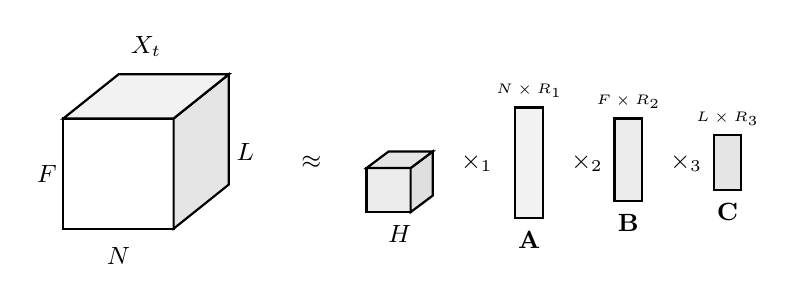
\begin{tikzpicture}[scale=0.7, every node/.style={font=\small}]
% Input tensor (3D cube)
\begin{scope}[shift={(0,0)}]
  \draw[thick, fill=white] (0,0,0) -- (2,0,0) -- (2,2,0) -- (0,2,0) -- cycle;
  \draw[thick, fill=gray!20] (2,0,0) -- (3,0.8,0) -- (3,2.8,0) -- (2,2,0) -- cycle;
  \draw[thick, fill=gray!10] (0,2,0) -- (2,2,0) -- (3,2.8,0) -- (1,2.8,0) -- cycle;
  \node at (1,-0.5,0) {$N$};
  \node at (3.3,1.4,0) {$L$};
  \node at (-0.3,1,0) {$F$};
  \node at (1.5,3.3,0) {$\mathbfcal{X}_t$};
\end{scope}

\node at (4.5,1.2) {$\approx$};

% Core tensor (smaller cube)
\begin{scope}[shift={(5.5,0.3)}]
  \draw[thick, fill=gray!15] (0,0,0) -- (0.8,0,0) -- (0.8,0.8,0) -- (0,0.8,0) -- cycle;
  \draw[thick, fill=gray!25] (0.8,0,0) -- (1.2,0.3,0) -- (1.2,1.1,0) -- (0.8,0.8,0) -- cycle;
  \draw[thick, fill=gray!20] (0,0.8,0) -- (0.8,0.8,0) -- (1.2,1.1,0) -- (0.4,1.1,0) -- cycle;
  \node at (0.6,-0.4,0) {$\mathbfcal{H}$};
\end{scope}

\node at (7.5,1.2) {$\times_1$};

% Factor A
\begin{scope}[shift={(8.2,0.2)}]
  \draw[thick, fill=gray!10] (0,0) rectangle (0.5,2);
  \node at (0.25,-0.4) {$\mathbf{A}$};
  \node at (0.25,2.3) {\tiny $N \times R_1$};
\end{scope}

\node at (9.5,1.2) {$\times_2$};

% Factor B
\begin{scope}[shift={(10,0.5)}]
  \draw[thick, fill=gray!15] (0,0) rectangle (0.5,1.5);
  \node at (0.25,-0.4) {$\mathbf{B}$};
  \node at (0.25,1.8) {\tiny $F \times R_2$};
\end{scope}

\node at (11.3,1.2) {$\times_3$};

% Factor C
\begin{scope}[shift={(11.8,0.7)}]
  \draw[thick, fill=gray!20] (0,0) rectangle (0.5,1);
  \node at (0.25,-0.4) {$\mathbf{C}$};
  \node at (0.25,1.3) {\tiny $L \times R_3$};
\end{scope}
\end{tikzpicture}
\caption{Mask-aware Tucker imputation for sparse fundamentals. To resolve missing entries without discarding sparse features, the incomplete input tensor $\mathbfcal{X}_t \in \mathbb{R}^{N \times F \times L}$ is approximated by a dense core tensor $\mathbfcal{H} \in \mathbb{R}^{40 \times 20 \times L}$ contracted with orthogonal factor matrices $\mathbf{A}$, $\mathbf{B}$, and $\mathbf{C}$ along each respective mode.}
\label{Fig:Tucker_Imputation}
\end{figure}

\subsection{Low-rank CP regression}
\label{Section:CP_Structured}

To stabilize the target tensor prior to estimation, we apply a within-firm centering analogous to fixed effects in panel econometrics. For each firm--feature pair, we compute a mask-aware temporal mean:
\begin{equation}
\mu_{ij} = \frac{\sum_{t} m_{tij}\, y_{tij}}{\sum_{t} m_{tij} + \varepsilon},
\end{equation}
where $m_{tij}$ is the observation indicator and $\varepsilon = 10^{-8}$ prevents division by zero. The centered residuals are further normalized by their observed root-mean-square,
\begin{equation}
s = \sqrt{\frac{1}{|\Omega|}\sum_{(t,i,j)\in\Omega}(y_{tij}-\mu_{ij})^2},
\end{equation}
where $\Omega = \{(t,i,j): m_{tij}=1\}$, yielding the scaled target $\tilde{y}_{tij} = m_{tij}(y_{tij}-\mu_{ij})/s$. Missing entries are set to zero in the scaled target.

We model the scaled, de-meaned target with a low-rank CANDECOMP/PARAFAC (CP) tensor regression. The coefficient tensor $\mathbfcal{W} \in \mathbb{R}^{N \times F \times L \times N \times F}$ admits the CP form
\begin{equation}
\mathbfcal{W} = \sum_{r=1}^{R} \mathbf{a}_r \circ \mathbf{b}_r \circ \mathbf{c}_r \circ \mathbf{d}_r \circ \mathbf{e}_r,
\end{equation}
where $\mathbf{a}_r \in \mathbb{R}^N$, $\mathbf{b}_r \in \mathbb{R}^F$, and $\mathbf{c}_r \in \mathbb{R}^L$ correspond to the input modes, while $\mathbf{d}_r \in \mathbb{R}^N$ and $\mathbf{e}_r \in \mathbb{R}^F$ correspond to the output modes of the $r$-th rank-one component. The prediction at time $t$ is obtained by inverting the centering and scaling:
\begin{equation}
\widehat{\mathbf{Y}}_t = \boldsymbol{\mu} + s \cdot \langle \mathbfcal{X}_t, \mathbfcal{W} \rangle \in \mathbb{R}^{N \times F},
\end{equation}
where $\boldsymbol{\mu} \in \mathbb{R}^{N \times F}$ is the firm--feature mean matrix and $s$ is the RMS scale defined above. Figure~\ref{Fig:CP_Regression} illustrates the structure of the CP regression model.

\begin{figure}[ht]
\centering
\resizebox{\linewidth}{!}{%
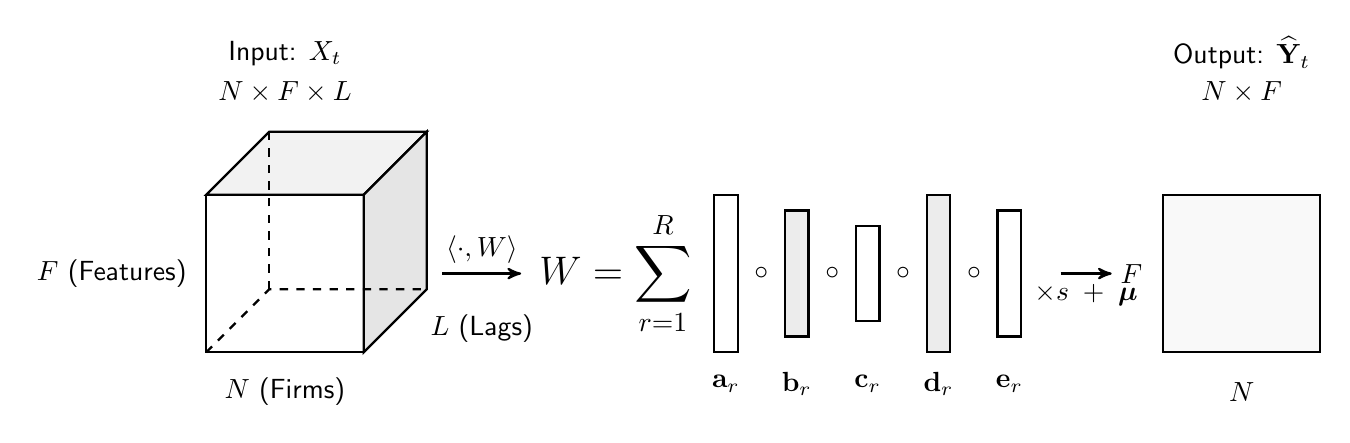
\begin{tikzpicture}[>=stealth', node distance=1.5cm, font=\sffamily]

% ===== Input tensor (3D cube) =====
\node at (1,3.8) {Input: $\mathbfcal{X}_t$};
\node at (1,3.3) {$N \times F \times L$};

\filldraw[fill=white, draw=black, thick] (0,0) rectangle (2,2);
\filldraw[fill=gray!10, draw=black, thick] (0,2) -- (0.8,2.8) -- (2.8,2.8) -- (2,2) -- cycle;
\filldraw[fill=gray!20, draw=black, thick] (2,0) -- (2.8,0.8) -- (2.8,2.8) -- (2,2) -- cycle;
\draw[dashed, thick] (0,0) -- (0.8,0.8) -- (2.8,0.8);
\draw[dashed, thick] (0.8,0.8) -- (0.8,2.8);

\node at (-1.2,1) {$F$ (Features)};
\node at (1,-0.5) {$N$ (Firms)};
\node at (3.5,0.3) {$L$ (Lags)};

% ===== Arrow: input -> contraction =====
\draw[->, thick] (3,1) -- (4,1) node[midway, above] {$\langle \cdot, \mathbfcal{W} \rangle$};

% ===== CP decomposition label =====
\node at (5.2,1) {\Large $\mathbfcal{W} = \displaystyle\sum_{r=1}^R$};

% ===== Five factor vectors (alternating white/gray) =====
\filldraw[fill=white, draw=black, thick] (6.45,0) rectangle (6.75,2);
\node at (6.6,-0.4) {$\mathbf{a}_r$};
\node at (7.05,1) {$\circ$};

\filldraw[fill=gray!15, draw=black, thick] (7.35,0.2) rectangle (7.65,1.8);
\node at (7.5,-0.4) {$\mathbf{b}_r$};
\node at (7.95,1) {$\circ$};

\filldraw[fill=white, draw=black, thick] (8.25,0.4) rectangle (8.55,1.6);
\node at (8.4,-0.4) {$\mathbf{c}_r$};
\node at (8.85,1) {$\circ$};

\filldraw[fill=gray!15, draw=black, thick] (9.15,0) rectangle (9.45,2);
\node at (9.3,-0.4) {$\mathbf{d}_r$};
\node at (9.75,1) {$\circ$};

\filldraw[fill=white, draw=black, thick] (10.05,0.2) rectangle (10.35,1.8);
\node at (10.2,-0.4) {$\mathbf{e}_r$};

% ===== Arrow: W -> output =====
\draw[->, thick] (10.85,1) -- (11.5,1) node[midway, below] {$\times s \;+\; \boldsymbol{\mu}$};

% ===== Output matrix (N x F) =====
\node at (13.15,3.8) {Output: $\widehat{\mathbf{Y}}_t$};
\node at (13.15,3.3) {$N \times F$};

\filldraw[fill=gray!5, draw=black, thick] (12.15,0) rectangle (14.15,2);
\node at (11.75,1) {$F$};
\node at (13.15,-0.5) {$N$};

\end{tikzpicture}%
}% end resizebox
\caption{Low-rank CP tensor regression model. The 5D weight tensor $\mathbfcal{W}$ is parameterized as a sum of $R$ rank-one components. The multilinear contraction $\langle \mathbfcal{X}_t, \mathbfcal{W} \rangle$ maps the historical 3D input ($N \times F \times L$) to a 2D next-quarter prediction ($N \times F$), which is then rescaled by $s$ and shifted by the firm--feature mean matrix $\boldsymbol{\mu}$.}
\label{Fig:CP_Regression}
\end{figure}

We estimate $\mathbfcal{W}$ via TensorLy \citep{kossaifi2019tensorly} by regularized least squares,
\begin{equation}
\min_{\mathbfcal{W}}
\sum_t \left\| \widetilde{\mathbf{Y}}_t - \langle \mathbfcal{X}_t, \mathbfcal{W} \rangle \right\|_F^2
+ \lambda \|\mathbfcal{W}\|_F^2,
\end{equation}
where $\widetilde{\mathbf{Y}}_t$ is the zero-filled, centered, RMS-scaled target defined above. Because TensorLy's CP solver does not accept observation masks, missing entries are set to zero prior to fitting; all evaluation at test time remains fully mask-aware. Hyperparameters---the rank $R \in \{5, \ldots, 50\}$ and regularization weight $\lambda \in [10^{-4}, 100]$---are tuned via Optuna on a rolling three-fold time-series split of the development data (80\% of windows).

\subsection{Ridge baseline and evaluation}
\label{Section:Baseline_Eval}

As a competitive baseline, we fit per-feature ridge regressions on vectorized lag windows. Both the CP and ridge models share the same within-firm centering described in Section~\ref{Section:CP_Structured}; the key distinction is that each ridge model is fitted independently for a single feature with its own regularization penalty, whereas the CP tensor shares one low-rank parameterization across all features simultaneously. For each feature $j \in \{1, \ldots, F\}$, let $\mathbf{y}^{(j)} \in \mathbb{R}^{T' N}$ denote the stacked target vector and $\mathbf{X} \in \mathbb{R}^{T' N \times FL}$ the design matrix formed by flattening the lag dimension. The per-feature model is
\begin{equation}
\mathbf{y}^{(j)} = \mathbf{X} \boldsymbol{\beta}^{(j)} + \boldsymbol{\mu}^{(j)} + \boldsymbol{\epsilon}^{(j)},
\end{equation}
where $\boldsymbol{\mu}^{(j)}$ contains the firm fixed effects for feature $j$.

Our pipeline computes mask-aware firm-feature means $\mu_i^{(j)}$ and models the de-meaned target directly---the classical \emph{within-transformation} in panel econometrics---removing the fixed effects before estimation and restoring them at prediction time.

To make the panel structure explicit, let $\mathbf{y}_i^{(j)} \in \mathbb{R}^{T'}$ denote the time-series target for firm~$i$ and feature~$j$, and let $\mathbf{X}_i \in \mathbb{R}^{T' \times FL}$ denote the firm's design matrix. The stacked panel regression groups observations by firm:
\begin{equation} \label{eq:ridge_panel}
\begin{bmatrix}
\mathbf{y}_{1}^{(j)} \\[2pt]
\hline
\\[-8pt]
\mathbf{y}_{2}^{(j)} \\[2pt]
\hline
\\[-8pt]
\vdots \\[2pt]
\hline
\\[-8pt]
\mathbf{y}_{N}^{(j)}
\end{bmatrix}
=
\begin{bmatrix}
\mathbf{X}_{1} \\[2pt]
\hline
\\[-8pt]
\mathbf{X}_{2} \\[2pt]
\hline
\\[-8pt]
\vdots \\[2pt]
\hline
\\[-8pt]
\mathbf{X}_{N}
\end{bmatrix}
\boldsymbol{\beta}^{(j)}
+
\begin{bmatrix}
\boldsymbol{\mu}_{1}^{(j)} \\[2pt]
\hline
\\[-8pt]
\boldsymbol{\mu}_{2}^{(j)} \\[2pt]
\hline
\\[-8pt]
\vdots \\[2pt]
\hline
\\[-8pt]
\boldsymbol{\mu}_{N}^{(j)}
\end{bmatrix}
+
\begin{bmatrix}
\boldsymbol{\epsilon}_{1}^{(j)} \\[2pt]
\hline
\\[-8pt]
\boldsymbol{\epsilon}_{2}^{(j)} \\[2pt]
\hline
\\[-8pt]
\vdots \\[2pt]
\hline
\\[-8pt]
\boldsymbol{\epsilon}_{N}^{(j)}
\end{bmatrix},
\end{equation}
where $\boldsymbol{\mu}_i^{(j)} \in \mathbb{R}^{T'}$ replicates firm~$i$'s historical mean across every time step. For a generic firm~$i$, the internal elements of $\mathbf{y}_i^{(j)}$ and $\mathbf{X}_i$ expand across time steps, features, and lags as:
\begin{equation} \label{eq:ridge_firm_elements}
\mathbf{y}_i^{(j)} =
\begin{bmatrix}
y_{i,\, t+1}^{(j)} \\
\vdots \\
y_{i,\, T'}^{(j)}
\end{bmatrix},
\qquad
\mathbf{X}_i =
\begin{bmatrix}
\overbrace{x_{i,\, t}^{(1)} \;\cdots\; x_{i,\, t}^{(F)}}^{\text{Lag } 1} & \cdots &
\overbrace{x_{i,\, t-L+1}^{(1)} \;\cdots\; x_{i,\, t-L+1}^{(F)}}^{\text{Lag } L} \\[4pt]
\vdots \quad \ddots \quad \vdots & \ddots & \vdots \quad \ddots \quad \vdots \\[4pt]
x_{i,\, T'\!-1}^{(1)} \;\cdots\; x_{i,\, T'\!-1}^{(F)} & \cdots &
x_{i,\, T'\!-L}^{(1)} \;\cdots\; x_{i,\, T'\!-L}^{(F)}
\end{bmatrix}.
\end{equation}

To ensure a rigorously competitive benchmark, ridge penalties are independently optimized for each feature via an inner three-fold time-series cross-validation from the candidate set $\alpha \in \{10^{-2}, 10^{-1}, 1, 10, 10^2, 10^3, 10^4\}$. This guarantees that the baseline is optimally tuned for the specific scale and variance of every individual fundamental feature. When a feature has too few observations (below an adaptive threshold), we revert to predicting the firm-mean baseline.

Performance is evaluated using a pooled, mask-aware coefficient of determination,
\begin{equation}
R^2 = 1 - \frac{\sum_{t,i,j} m_{tij} (y_{tij} - \widehat{y}_{tij})^2}
{\sum_{t,i,j} m_{tij} (y_{tij} - \bar{y})^2},
\end{equation}
with $\bar{y}$ the mean of observed entries. We also compute per-feature $R^2$ values to identify which fundamentals are most predictable. To assess whether CP regression systematically outperforms ridge, we estimate AR(1) persistence per feature and examine the association between persistence and the performance gap ($\Delta = R^2_{\mathrm{CP}} - R^2_{\mathrm{Ridge}}$) using Spearman correlation and paired Wilcoxon tests with Benjamini--Hochberg adjustment for multiple comparisons.

\subsection{Empirical results}
\label{Section:Predictive_Results}

We now present the comparative forecasting performance of the CP tensor regression against the highly structured ridge baseline. Table~\ref{Tab:CP_Ridge_Results} reports the pooled, mask-aware coefficient of determination ($R^2$) on the held-out test (20\%) set for each input scaling mode (\textsc{Unscaled} and \textsc{Normalized}) and lookback horizon ($L \in \{2, 4\}$). Both models share the same within-firm centering (Section~\ref{Section:CP_Structured}), but the ridge baseline enjoys two structural advantages: (i)~a separate, independently fitted model for every feature, whereas the tensor shares a single low-rank parameterization across all features simultaneously; and (ii)~per-feature regularization penalties selected by inner cross-validation, whereas the tensor uses one global set of hyperparameters. Despite these advantages, the CP tensor matches or exceeds the ridge baseline across all configurations, demonstrating that the cross-feature multilinear structure it captures is genuinely predictive and cannot be replicated by even a well-tuned collection of independent regressions. To further understand where the tensor formulation provides the most value, Table~\ref{Tab:Persistence_Stats} summarizes the feature-level AR(1) persistence analysis, quantifying the statistical significance of the performance gap ($\Delta$) using Benjamini--Hochberg adjusted $p$-values.

Table~\ref{Tab:CP_Ridge_Results} shows that the CP tensor regression outperforms the ridge baseline across all four configurations, with the largest gains emerging under \textsc{Normalized} scaling at $L=4$ ($\Delta = +0.028$). The consistent positive deltas demonstrate that the multilinear structure captured by the 5D weight tensor provides genuine predictive value beyond what per-feature linear models can achieve. Notably, the \textsc{Normalized} mode yields the strongest CP performance overall (Test $R^2 = 0.784$ at $L=4$), confirming that RMS normalization removes magnitude-driven scaling artifacts and allows the tensor to focus on the underlying cross-firm, cross-feature dynamics.

\begin{table}[!htbp]
\centering
\caption{CP tensor regression versus ridge baseline: pooled $R^2$ on held-out test (20\%) set.}
\label{Tab:CP_Ridge_Results}
\begin{tabular}{llcccc}
\toprule
Mode & $L$ & Ridge Test $R^2$ & CP Test $R^2$ & $\Delta$ \\
\midrule
\textsc{Unscaled}   & 2 & 0.760 & \textbf{0.778} & $+0.018$ \\
\textsc{Unscaled}   & 4 & 0.758 & \textbf{0.766} & $+0.008$ \\
\textsc{Normalized} & 2 & 0.750 & \textbf{0.768} & $+0.018$ \\
\textsc{Normalized} & 4 & 0.756 & \textbf{0.784} & $+0.028$ \\
\bottomrule
\end{tabular}
\end{table}

Table~\ref{Tab:Persistence_Stats} confirms that the CP tensor provides a statistically significant predictive advantage over the ridge baseline in three of four configurations (Wilcoxon $p_{\mathrm{adj}}<0.01$). The relationship between AR(1) persistence and the performance gap is mode-dependent: under \textsc{Normalized} scaling, the CP advantage concentrates on more persistent features ($r=0.468$, $p_{\mathrm{adj}}=0.042$ at $L=2$), while under \textsc{Unscaled} scaling at $L=4$ the pattern reverses sharply ($r=-0.835$, $p_{\mathrm{adj}}<10^{-5}$), with the tensor excelling on less persistent series. This mode dependence suggests that RMS normalization fundamentally alters which cross-feature dynamics the tensor exploits, and that the multilinear structure captures predictive information inaccessible to per-feature regressions regardless of the persistence regime.

\begin{table}[!htbp]
\centering
\caption{Persistence diagnostics and statistical significance (Benjamini--Hochberg adjusted $p$-values).}
\label{Tab:Persistence_Stats}
\begin{tabular}{llcccc}
\toprule
Mode & $L$ & Mean $\Delta$ & Spearman $r$ & Spearman $p_{\mathrm{adj}}$ & Wilcoxon $p_{\mathrm{adj}}$ \\
\midrule
\textsc{Unscaled}   & 2 & $+0.152$ & 0.395 & 0.075 & \textbf{0.0002} \\
\textsc{Unscaled}   & 4 & $+0.030$ & $-0.835$ & \textbf{0.000002} & 0.197 \\
\textsc{Normalized} & 2 & $+0.168$ & 0.468 & \textbf{0.042} & \textbf{0.002} \\
\textsc{Normalized} & 4 & $+0.124$ & 0.054 & 0.802 & \textbf{0.0000005} \\
\bottomrule
\end{tabular}
\end{table}




%%%%%%%%%%%%%%%%%%%%%%%%%%%%%%%%%%%%%%%%%%%%%%%%%%%%%%%%%%%%%%%%%%%%%%%%%%%%%%%%%%%%%%%%%%%%%%%%%%%%%%%%%%%%%%%%%%%%%%%%%%%%%%%%%%%%%%%%


\section{Conclusion}

In this paper, we introduced a novel, tensor-based framework for modeling and forecasting firm-level fundamentals. By constructing the Market Fundamentals Index (MFI), we provided a structural lens into market-wide volatility, successfully demonstrating that fluctuations in accounting fundamentals are statistically dependent on price-based chaos (FCIX).

Building upon this structural relationship, we developed a rigorous predictive pipeline that resolves real-world data sparsity via mask-aware Tucker imputation. We demonstrated that a low-rank CANDECOMP/PARAFAC (CP) tensor regression---when properly controlled with firm-by-feature fixed effects---can effectively exploit the multilinear dynamics between historical lags, firm heterogeneity, and cross-feature interactions. Ultimately, this framework establishes a robust foundation for systematically evaluating the predictability of quarterly fundamentals, paving the way for future extensions incorporating broader asset universes and macroeconomic covariates.

%%%%%%%%%%%%%%%%%%%%%%%%%%%%%%%%%%%%%%%%%%%%%%%%%%%%%%%%%%%%%%%%%%%%%%%%%%%%%%%%%%%%%%%%%%%%%%%%%%%%%%%%%%%%%%%%%%%%%%%%%%%%%%%%%%%%%%%%




%\subsection{Block-wise Granger Causality}
%\label{Section:7_4}
%Let us first assume that the market fundamentals index is already at our disposal. Hence, we may devote the remainder of this section to discover the existence of causal relations from \textit{policy uncertainty indexes} to $\mathrm{FCIX}_t$ by further taking into account the assets' fundamentals information. To this end, we first formulate a conditional null hypothesis and then perform a \textit{$1$-step block-wise Granger causality} test to identify and characterize possible causal relations. A reason for choosing only $1$-step-ahead Granger causality tests, is due to the observation that selecting a minimal possible time-horizon size (i.e., $h=1$ or equivalently, one single quarter of the time unit) could be sufficient to capture potential changes in macroeconomic factors and assets' fundamentals that may influence the stock market trends. In addition, inspection of  \ref{Fig:Cross_Corr_Quarterly} supports our choice for the size of time-horizon, whereby it is observed that the maximum cross-correlation between $\mathrm{FCIX}_t$ and $\mathrm{MFI}_t$ occurs at $1$-lag quarter having its value to be $73.378\%$.
%
%Denote by $\mathcal{J}_{t,\mathtt{Q}}^{\mathtt{PRC}} = \mathscr{F}_{\mathrm{FCIX},t}$ the set of known information for $\mathrm{FCIX}_t$ up to a quarter of time unit $t$. Also, we will slightly abuse the notation, by using $\mathbf{F}_t$ to represent $\mathrm{FCIX}_t$. Let us now define the following quarterly multivariate time series
%\begin{equation*}
%	\mathbf{U}_t = \left( \mathrm{VIX}_t, \mathrm{MFI}_t \right)^\intercal  ,
%\end{equation*}
%and
%\begin{equation*}
%	\resizebox{1\hsize}{!}  { $\mathbf{W}_t = \left( \mathrm{EMV}_t, \mathrm{EPU}_t, \mathrm{MON}_t, \mathrm{FIS}_t, \mathrm{TAX}_t, \mathrm{GOV}_t, \mathrm{HLTH}_t, \mathrm{SEC}_t, \mathrm{ENT}_t, \mathrm{GREG}_t, \mathrm{FREG}_t, \mathrm{TRD}_t, \mathrm{CPI}_t \right)^\intercal $}  ,
%\end{equation*}
%with their respective sets of the known information represented by $ \mathscr{F}_{\mathrm{VIX},t} \bigotimes \mathscr{F}_{\mathrm{MFI},t} $, and  $$ \mathcal{J}_{t,\mathtt{Q}}^{\mathtt{NEWS}} = \bigotimes_{k=1}^K \mathscr{F}_{\mathbf{W}_{k},t}  ,$$ where $K=13$.
%
%Next, we would like to test whether the group of individual univariate components of $\mathbf{W}_t$ are not a $1$-step Granger cause of $\mathrm{FCIX}_t$, given the information on the respective components of $\mathbf{U}_t$. However, since both components of $\mathbf{U}_t$ are statistically dependent on $\mathrm{FCIX}_t$, i.e., $\mathrm{VIX}_t$ dependents through cointegration (e.g., see \ref{Section:5_2}) and $\mathrm{MFI}_t$ by implications of the independence tests executed in \ref{Section:7_3}, then possibilities of inferring spurious causalities would potentially be eliminated if these common dependencies ($\mathrm{VIX}_t$ and $\mathrm{FCIX}_t$) are \textit{conditioned out}.
%
%To this end, we express the joint distribution of the multivariate processes $(\mathbf{F}_t,\mathbf{W}_t,\mathbf{U}_t)^\intercal$ in VAR($p$) form as follows:
%\begin{equation}
%	\label{Eq:VAR_MFI}
%	\begin{pmatrix}
%		\mathbf{F}_t \\
%		\mathbf{W}_t \\
%		\mathbf{U}_t 
%	\end{pmatrix} 
%	= \nsum\limits_{k=1}^p
%	\begin{pmatrix}
%		b_{ff,k} & b_{fw,k} & b_{fu,k} \\
%		b_{wf,k} & b_{ww,k} & b_{wu,k} \\
%		b_{uf,k} & b_{uw,k} & b_{uu,k}
%	\end{pmatrix} 
%	\begin{pmatrix}
%		\mathbf{F}_{t-k} \\
%		\mathbf{W}_{t-k} \\
%		\mathbf{U}_{t-k} 
%	\end{pmatrix}
%	+
%	\begin{pmatrix}
%		{\epsilon}_{f,t} \\
%		\boldsymbol{\epsilon}_{w,t} \\
%		\boldsymbol{\epsilon}_{u,t} 
%	\end{pmatrix}  .
%\end{equation}
%Here, the residual variance-covariance matrix of the error vectors takes on a form as follows:
%\begin{equation}
%	\boldsymbol{\Sigma} = 
%	\mathrm{cov}
%	\begin{pmatrix}
%		{\epsilon}_{f,t} \\
%		\boldsymbol{\epsilon}_{w,t} \\
%		\boldsymbol{\epsilon}_{u,t} 
%	\end{pmatrix} 
%	= 
%	\begin{pmatrix}
%		{\Sigma}_{ff} & \boldsymbol{\Sigma}_{fw} & \boldsymbol{\Sigma}_{fu} \\
%		\boldsymbol{\Sigma}_{wf} & \boldsymbol{\Sigma}_{ww} & \boldsymbol{\Sigma}_{wu} \\
%		\boldsymbol{\Sigma}_{uf} & \boldsymbol{\Sigma}_{uw} & \boldsymbol{\Sigma}_{uu}
%	\end{pmatrix}  . 
%\end{equation}
%Note that that the relation given by \ref{Eq:VAR_MFI} does not involve neither the shift nor a linear trend components due to the fact that $\mathrm{FCIX}_t$ is an $I(1)$ process with no shift or linear trend, as per \ref{Section:3_2}. Subsequently, by analogy to \ref{Section:6}, we express the \textit{unrestricted} and \textit{restricted} regression models by
%\begin{equation}
%	\mathbf{F}_t = \sum\limits_{k=1}^p b_{ff,k} \mathbf{F}_{t-k} + \sum\limits_{k=1}^p b_{fw,k} \mathbf{W}_{t-k}  + \sum\limits_{k=1}^p b_{fu,k} \mathbf{U}_{t-k} + {\epsilon}_{f,t}  ,
%\end{equation}
%and
%\begin{equation}
%	\mathbf{F}_t = \sum\limits_{k=1}^p b_{ff,k}^{'} \mathbf{F}_{t-k} + \sum\limits_{k=1}^p b_{fu,k}^{'} \mathbf{U}_{t-k} + {\epsilon}_{f,t}^{'}  ,
%\end{equation}
%respectively, where the variables used for conditioning that are contained in $\mathbf{U}_t$, are present in both of the above models. 
%
%In turn, the null hypothesis on no causality is formulated as follows:
%\begin{equation*}
%	\mathrm{H}_{0,\mathtt{Q}}^{\mathtt{NEWS}} : \forall k\in\{1,2\dots,p\}, b_{wf,k} = 0  ,
%\end{equation*}
%whose corresponding alternative hypothesis is:
%\begin{equation*}
%	\mathrm{H}_{1,\mathtt{Q}}^{\mathtt{NEWS}} : \exists k\in\{1,2\dots,p\}, b_{wf,k} \neq 0  .
%\end{equation*}
%Similar to \ref{EQ:GC_Measure}, the test statistic based on the generalized variance of the regression models is utulized, which estimates the \textit{model prediction error} and is given by the following \text{log-likelihood ratio}:
%\begin{equation}
%	\label{EQ:GC_Measure_Conditional}
%	\mathrm{GC}_{\mathbf{W}_t\overset{h=1}{\nrightarrow} \mathbf{F}_t|\mathbf{U}_t} = \log \frac{|\Sigma_{ff}^{'}|}{|\Sigma_{ff}|}  \cdot
%\end{equation}
%
%\ref{Blockwise_News_Results} summarizes the results obtained for testing $\mathrm{H}_{0,\mathtt{Q}}^{\mathtt{NEWS}}$. Both $\chi^2$ and $F$ underlying distributions for the test statistics were considered. As per these results, there is no sufficient evidence to reject the null hypothesis $\mathrm{H}_{0,\mathtt{Q}}^{\mathtt{NEWS}}$ at $1\%$ level of significance using either of these test statistics. In turn, this implies that the mutual quarterly price changes of the assets are $1$-step Granger caused by news-based uncertainty indexes, given the known information sets pertaining to $\mathrm{VIX}_t$ and $\mathrm{MFI}_t$. In other words, the null hypothesis does not get rejected w.r.t. the known information set  $\mathcal{J}_{t,\mathtt{Q}}^{\mathtt{PRC}} \bigoplus \mathcal{J}_{t,\mathtt{Q}}^{\mathtt{NEWS}} | \mathscr{F}_{\mathrm{VIX},t} \bigotimes \mathscr{F}_{\mathrm{MFI},t}.$
%
%\begin{table}[ht]
%	\centering
%	\footnotesize
%	\caption{Results of Granger causality test for $\mathrm{H}_{0,\mathtt{Q}}^{\mathtt{NEWS}}$.}
%	\label{Blockwise_News_Results}
%	\begin{tabular}{lcc} 
%		\toprule
%		& $\chi^2$-test & $F$-test \\
%		\midrule
%		p-value         & 0.129   & 0.234 \\
%		Test statistics & 63.663  & 1.224 \\
%		\addlinespace
%		\textbf{Critical values} & & \\
%		\quad 1\% level  & 78.660  & 1.923 \\
%		\quad 5\% level  & 69.832  & 1.585 \\
%		\quad 10\% level & 65.422  & 1.431 \\
%		\bottomrule
%	\end{tabular}
%\end{table}
%
%	
%	Moreover, it is very important to investigate the impacts of news-based information ($\mathcal{J}_{t,\mathtt{Q}}^{\mathtt{NEWS}}$) augmented with the fundamentals' information ($\mathscr{F}_{\mathrm{MFI},t}$), on the price-generating mechanisms of the assets. As we may assume without the loss of generality that such an augmented set of information alongside the price-related sets of known information ($\mathscr{F}_{\mathrm{FCIX},t}$ and $\mathscr{F}_{\mathrm{VIX},t}$) contains all the \textit{publicly known information} about the assets. To this end, we reshape the configuration of the elements contained in the multivariate time series $\mathbf{W}_t$ and $\mathbf{U}_t$, and introduce two new time series
%	\begin{equation*}
%		\mathbf{\widetilde{U}}_t =  \mathrm{VIX}_t   ,
%	\end{equation*}
%	and
%	\begin{equation*}
%		\resizebox{1\hsize}{!}  { $\mathbf{\widetilde{W}}_t = \left( \mathrm{MFI}_t, \mathrm{EMV}_t, \mathrm{EPU}_t, \mathrm{MON}_t, \mathrm{FIS}_t, \mathrm{TAX}_t, \mathrm{GOV}_t, \mathrm{HLTH}_t, \mathrm{SEC}_t, \mathrm{ENT}_t, \mathrm{GREG}_t, \mathrm{FREG}_t, \mathrm{TRD}_t, \mathrm{CPI}_t \right)^\intercal $} ,
%	\end{equation*}
%	whose respective sets of known information are represented by $ \mathscr{F}_{\mathrm{VIX},t}  $ and $$ \mathcal{J}_{t,\mathtt{Q}}^{\mathtt{PUB}} = \left( \bigotimes_{k=2}^{K^{'}} \mathscr{F}_{\mathbf{\widetilde{W}}_{k},t} \right) \bigoplus \mathscr{F}_{\mathrm{MFI},t}  , $$ where $K{'}=14$. Thereafter, the corresponding \textit{unrestricted} and \textit{restricted} regression models are re-derived, but for this time it is to be done by substituting $\mathbf{\widetilde{U}}_t$ for $\mathbf{U}_t$ and $\mathbf{\widetilde{W}}_t$ for $\mathbf{W}_t$. Subsequently, we reformulate a null hypothesis as follows:
%	\begin{equation*}
%		\mathrm{H}_{0,\mathtt{Q}}^{\mathtt{PUB}} : \forall k\in\{1,2\dots,p\},  \tilde{b}_{\tilde{w}f,k} = 0  ,
%	\end{equation*}
%	and test it versus the following alternative:
%	\begin{equation*}
%		\mathrm{H}_{1,\mathtt{Q}}^{\mathtt{PUB}} : \exists k\in\{1,2\dots,p\},  \tilde{b}_{\tilde{w}f,k} \neq 0  .
%	\end{equation*}
%	The corresponding test statistic is further given by
%	\begin{equation}
%		\label{EQ:GC_Measure_Conditional_Pub}
%		\mathrm{GC}_{\mathbf{\widetilde{W}}_t\overset{h=1}{\nrightarrow} \mathbf{F}_t|\mathbf{\widetilde{U}}_t} = \log \frac{|\widetilde{\Sigma}_{ff}^{'}|}{|\widetilde{\Sigma}_{ff}|}  \cdot
%	\end{equation}
%	
%	
%\begin{table}[ht]
%	\centering
%	\footnotesize
%	\caption{Results of Granger causality test for $\mathrm{H}_{0,\mathtt{Q}}^{\mathtt{PUB}}$.}
%	\label{Blockwise_Public_Results}
%	\begin{tabular}{lcc} 
%		\toprule
%		& $\chi^2$-test & $F$-test \\
%		\midrule
%		p-value         & 0.014   & 0.134 \\
%		Test statistics & 98.603  & 1.409 \\
%		\addlinespace
%		\textbf{Critical values} & & \\
%		\quad 1\% level  & 100.425 & 2.072 \\
%		\quad 5\% level  & 90.531  & 1.665 \\
%		\quad 10\% level & 85.527  & 1.486 \\
%		\bottomrule
%	\end{tabular}
%\end{table}
%
%
%According to the results presented in \ref{Blockwise_Public_Results}, there is insufficient evidence to reject the null hypothesis that the market fundamentals index alongside newschapter-based uncertainty indexes do not $1$-step Granger cause $\mathrm{FCIX}_t$ at $1\%$ level of significance, i.e., the null hypothesis does not get rejected w.r.t. the known information set $\mathcal{J}_{t,\mathtt{Q}}^{\mathtt{PRC}} \bigoplus \mathcal{J}_{t,\mathtt{Q}}^{\mathtt{PUB}} | \mathscr{F}_{\mathrm{VIX},t} $. In  turn, this implies that the quarterly price changes exhibited by the mutual behavior of the assets in the stock market are $1$-step Granger caused by macroeconomic and/or policy uncertainty news as well as the fundamentals-related information. 
%
%
%
%




%%%%%%%%%%%%%%%%%%%%%%%%%%%%%%%%%%%%%%%%%%%%%%%%%%%%%%%%%%%%%%%%%%%%%%%%%%%%%%%%%%%%%%%%%%%%%%%%%%%%%%%%%%%%%%%%%%%%%%%%%%%%%%%%%%%%%%%%
%%%%%%%%%%%%%%%%%%%%%%%%%%%%%%%%%%%%%%%%%%%%%%%%%%%%%%%%%%%%%%%%%%%%%%%%%%%%%%%%%%%%%%%%%%%%%%%%%%%%%%%%%%%%%%%%%%%%%%%%%%%%%%%%%%%%%%%%
%%%%%%%%%%%%%%%%%%%%%%%%%%%%%%%%%%%%%%%%%%%%%%%%%%%%%%%%%%%%%%%%%%%%%%%%%%%%%%%%%%%%%%%%%%%%%%%%%%%%%%%%%%%%%%%%%%%%%%%%%%%%%%%%%%%%%%%%




































%%%%%%%%%%%%%%%%%%%%%%%%%%%%%%%%%%%%%%%%%%%%%%%%%%%%%%%%%%%%%%%%%%%%%%%%%%%%%%%%%%%%%%%%%%%%%%%%%%%%%%%%%%%%%%%%%%%%%%%%%%%%%%%%%%%%%%%%
%%%%%%%%%%%%%%%%%%%%%%%%%%%%%%%%%%%%%%%%%%%%%%%%%%%%%%%%%%%%%%%%%%%%%%%%%%%%%%%%%%%%%%%%%%%%%%%%%%%%%%%%%%%%%%%%%%%%%%%%%%%%%%%%%%%%%%%%
%%%%%%%%%%%%%%%%%%%%%%%%%%%%%%%%%%%%%%%%%%%%%%%%%%%%%%%%%%%%%%%%%%%%%%%%%%%%%%%%%%%%%%%%%%%%%%%%%%%%%%%%%%%%%%%%%%%%%%%%%%%%%%%%%%%%%%%%


%\section{The Efficient Market Hypothesis}
%\label{Section:8}
%In the last section of our chapter, we employ the previously developed tools and concepts and concentrate on the long-standing \textit{efficient market hypothesis} (EMH). The literature on EMH and its definition is vast and extensive; we refer the interested reader to \citep{degutis2014efficient,gabriela2015efficient,naseer2015efficient, lehmann1990fads, stein1989efficient, shi2018should}, to list a few. However, in some broad sense, EMH stipulates that market prices fully reflect all available information, further implying that the sequences of the asset price changes would behave in a more random manner in the case where the market exhibits larger degrees of efficiency, to the extent that in a completely efficient market the price changes would be completely unpredictable. 
%
%One possible approach that we follow in this section is to formulate the EMH using the notion of the financial chaos index. Note that such a possibility stems from the remark made in \ref{Section:3} where it was discussed that $\mathrm{FCIX}_t$ could potentially be considered as a consistent and robust estimator of the market volatility. Hence, we present three versions of the EMH formulated in terms of the financial chaos index which are in the same spirit as to the definitions provided in \citep{jensen1978some}. 
%
%We stress the fact that failure to reject EMH, or alternatively accept it, has few implications for efficiency of the market price formations insofar as there is insufficient existence of a thorough and explicit economic model accounting for price-generating mechanisms, e.g., see \citep{lo1988stock} for similar arguments. State it differently, the price formation of the assets in the stock market during the considered time period is deemed efficient only in relation to our underlying tensorial economic model.
%
%Throughout, we will use $\mathcal{J}_{t,\mathtt{D}}$, $\mathcal{J}_{t,\mathtt{M}}$ and $\mathcal{J}_{t,\mathtt{Q}}$ to denote the sets of some known information per daily, monthly and quarterly time frequencies, respectively.
%
%
%%%%%%%%%%%%%%%%%%%%%%%%%%%%%%%%%%%%%%%%%%%%%%%%%%%%%%%%%%%%%%%%%%%%%%%%%%%%%%%%%%%%%%%%%%%%%%%%%%%%%%%%%%%%%%%%%%%%%%%%%%%%%%%%%%%%%%%%%
%
%\subsection{Weak EMH}
%\label{Section:8_1}
%
%A \textit{weak} form of the EMH stipulates that given the past and present values of the assets, it is impossible to predict their future values. The weak form of EMH can be defined in terms of our developed financial chaos index as follows:
%\begin{definition}[Weak EMH]
%	Let $\mathcal{J}_t^{\mathtt{PRC}}$ denote a set of known information for financial chaos index at time $t$. Assume without the loss of generality that $\mathcal{J}_t^{\mathtt{PRC}}$ entails all the known information pertaining to the observed historical prices of $N$ particular assets up to time $t\in \mathcal{T}$. Then, the market is said to be weakly efficient w.r.t. $\mathcal{J}_t^{\mathtt{PRC}}$ if $\mathrm{FCIX}_t$ is a random walk. 
%\end{definition}
%
%As per our analysis and discussion given in \ref{Section:3_4}, the daily $\mathrm{FCIX}_t$ did not satisfy the conditions for being a random walk. Thus, we may conclude that the stock market during the time period January $1990$-December $2019$ was weakly inefficient w.r.t. $\mathcal{J}_{t,\mathtt{D}}^{\mathtt{PRC}}$. On the contrary, for the monthly and quarterly time frequencies, there exist insufficient evidence to reject the random walk hypotheses on $\mathrm{FCIX}_t$. As a consequence, the stock market during the given time period can be regarded as being weakly efficient w.r.t. both $\mathcal{J}_{t,\mathtt{M}}^{\mathtt{PRC}}$ and $\mathcal{J}_{t,\mathtt{Q}}^{\mathtt{PRC}}$ at $1\%$ level of significance.
%
%
%%%%%%%%%%%%%%%%%%%%%%%%%%%%%%%%%%%%%%%%%%%%%%%%%%%%%%%%%%%%%%%%%%%%%%%%%%%%%%%%%%%%%%%%%%%%%%%%%%%%%%%%%%%%%%%%%%%%%%%%%%%%%%%%%%%%%%%%%
%
%
%\subsection{Potent EMH}
%\label{Section:8_2}
%
%Here, we introduce a concept of the \textit{potent} EMH to investigate whether news-based uncertainty indexes Granger cause the past and current values of the assets. To be more precise, if the news-based information sets really influence the prices in an \textit{efficient market}, then there should only exist instantaneous Granger causal relations from news-based information on the prices. In other words, one would not expect to find any strictly Granger causal relation from such news-based information on the prices in an \textit{efficient market}, for any strictly causal relation would indicate that there already exist news-based information which have not been utilized efficiently, e.g., compare to \citep{kirchgassner2012introduction}. This can be made rigorous by using the financial chaos index. Specifically, the potent EMH can be defined as follows:
%
%\begin{definition}[Potent EMH]
%	
%	Let $\mathcal{J}_t^{\mathtt{PRC}}$ and $\mathcal{J}_t^{\mathtt{NEWS}}$ denote sets of known information for financial chaos index and a collection of news-based uncertainty indexes at time $t$, respectively. Assume without the loss of generality that the set $\mathcal{J}_t^{\mathtt{PRC}} \bigoplus \mathcal{J}_t^{\mathtt{NEWS}}$ entails all the known information pertaining to the observed historical prices of specific $N$ assets as well as the macroeconomic and various types of policy uncertainty news up to time $t\in \mathcal{T}$. Then, the market is said to be potently efficient w.r.t. $\mathcal{J}_t^{\mathtt{PRC}}\bigoplus \mathcal{J}_t^{\mathtt{NEWS}}$ if $\mathrm{FCIX}_t$ is a random walk, and there is no strictly Granger causal relation from the collection of news-based policy uncertainty indexes on $\mathrm{FCIX}_t$.
%\end{definition}
%
%As per the above definition, we may state that the U.S. stock market during the time period January $1990$-December $2019$ was potently inefficient w.r.t. $\mathcal{J}_{t,\mathtt{D}}^{\mathtt{PRC}}\bigoplus \mathcal{J}_{t,\mathtt{D}}^{\mathtt{NEWS}}$, since the daily $\mathrm{FCIX}_t$ during the considered time period did not satisfy the conditions for being a random walk, and further the null hypothesis that daily $\mathrm{FCIX}_t$ was time-lagged (strictly) Granger caused by news-based uncertainty indexes at all the $1\%$ levels of significance (e.g., see \ref{Section:6_2} for more details). On the other hand, it was shown that for the monthly and quarterly data, $\mathrm{FCIX}_t$ was a random walk, and also that the news-based policy uncertainty indexes did not strictly Granger cause $\mathrm{FCIX}_t$ (e.g., see \ref{Section:6_3,Section:7_4} for more information). Therefore, the stock market during the given time period could be proclaimed to have been potently efficient w.r.t. $\mathcal{J}_{t,\mathtt{M}}^{\mathtt{PRC}}\bigoplus \mathcal{J}_{t,\mathtt{M}}^{\mathtt{NEWS}}$ and $\mathcal{J}_{t,\mathtt{Q}}^{\mathtt{PRC}}\bigoplus \mathcal{J}_{t,\mathtt{Q}}^{\mathtt{NEWS}}$ at $1\%$ level of significance.
%
%
%%%%%%%%%%%%%%%%%%%%%%%%%%%%%%%%%%%%%%%%%%%%%%%%%%%%%%%%%%%%%%%%%%%%%%%%%%%%%%%%%%%%%%%%%%%%%%%%%%%%%%%%%%%%%%%%%%%%%%%%%%%%%%%%%%%%%%%%%
%
%
%\subsection{Semi-strong EMH}
%\label{Section:8_3}
%
%Our final goal is to investigate whether all the publicly known information Granger cause the past and current values of the assets. By assuming that the set of all publicly known information is comprised of news-based information augmented with the information pertaining to fundamental features of the assets, a \textit{semi-strong} version of EMH can be made rigorous using the notion of the financial chaos index as follows:
%
%\begin{definition}[Semi-strong EMH]
%	
%	Let $\mathcal{J}_t^{\mathtt{PRC}}$ and $\mathcal{J}_t^{\mathtt{PUB}}$ denote sets of known information for financial chaos index and   publicly accessible information at time $t$, respectively. Assume without the loss of generality that the set $\mathcal{J}_t^{\mathtt{PRC}} \bigoplus \mathcal{J}_t^{\mathtt{PUB}}$ entails all the known information pertaining to the observed historical prices of specific $N$ assets as well as the publicly accessible information provided by the news-based sources and assets' fundamentals up to time $t\in \mathcal{T}$. Then, the market is said to be semi-strongly efficient w.r.t. $\mathcal{J}_t^{\mathtt{PRC}}\bigoplus \mathcal{J}_t^{\mathtt{PUB}}$ if $\mathrm{FCIX}_t$ is a random walk, and there is no strictly Granger causal relation from the collection of news-based policy uncertainty indexes and/or market fundamental index on $\mathrm{FCIX}_t$.
%\end{definition}
%
%For the daily and monthly data, the semi-strong form of EMH basically reduces to the potent version of EMH since the information pertaining to the fundamentals of assets are typically accessible to agents only per quarterly or annual time frequencies, i.e., $\mathcal{J}_{t,\mathtt{D}}^{\mathtt{PUB}}=\mathcal{J}_{t,\mathtt{D}}^{\mathtt{NEWS}}$ and $\mathcal{J}_{t,\mathtt{M}}^{\mathtt{PUB}}=\mathcal{J}_{t,\mathtt{M}}^{\mathtt{NEWS}}$. Thus, we may conclude that the U.S. stock market was semi-strongly inefficient w.r.t. $\mathcal{J}_{t,\mathtt{D}}^{\mathtt{PRC}}\bigoplus \mathcal{J}_{t,\mathtt{D}}^{\mathtt{PUB}}$ at the significance level $1\%$, while the market was semi-strongly efficient w.r.t. $\mathcal{J}_{t,\mathtt{M}}^{\mathtt{PRC}}\bigoplus \mathcal{J}_{t,\mathtt{M}}^{\mathtt{PUB}}$ at $1\%$ level of significance. 
%
%However, the set $\mathcal{J}_{t,\mathtt{Q}}^{\mathtt{PUB}}$ is comprised of the known information on collection of  policy uncertainty indexes together with the market fundamentals index. Since the quarterly $\mathrm{FCIX}_t$ was shown to be a random walk and time-lagged Granger causal relations did not exist from the news-based policy uncertainty indexes and/or market fundamental index on $\mathrm{FCIX}_t$ (e.g., see \ref{Section:7_4} for more details), the market during the time period January $1990$-December $2019$ could be claimed to have been semi-strongly efficient w.r.t. $\mathcal{J}_{t,\mathtt{Q}}^{\mathtt{PRC}}\bigoplus \mathcal{J}_{t,\mathtt{Q}}^{\mathtt{PUB}}$ at $1\%$ level of significance.
%
%
%
%
%






%%===========================================================================================%%
%% If you are submitting to one of the Nature Portfolio journals, using the eJP submission   %%
%% system, please include the references within the manuscript file itself. You may do this  %%
%% by copying the reference list from your .bbl file, paste it into the main manuscript .tex %%
%% file, and delete the associated \verb+\bibliography+ commands.                            %%
%%===========================================================================================%%
\newpage
\bibliography{references}% common bib file
%% if required, the content of .bbl file can be included here once bbl is generated
%%\input sn-article.bbl


\end{document}





%%%%%%%%%%%%%%%%%%%%%%%%%%%%%%%%%%%%%%%%%%%%%%%%%%%%%%%%%%%%%%%%%%%%%%%%%%%%%%%%%%%%%%%%%%%%%%%%%%%%%%%%%%%%%%%%%%%%%%%%%%%%%%%%%%%%%%%%%
%
%\section{Encoding Fundamentals Information}
%\label{Section:Funadamentals}
%
%In this section, we develop a methodology for embedding stock market fundamentals into structured representations and identifying a subset of features that preserves the latent economic structure of the market. The ultimate objective is to facilitate the construction of a volatility index grounded in fundamental information. The selected features are required to align with a reference taxonomy of economic activity, namely the Global Industry Classification Standard (GICS), thus providing a bridge between qualitative categorization and quantitative representation.
%
%\subsection{Feature Selection}
%\label{Section:Feature_Selection}
%
%Let $S = \{S_1, S_2, \ldots, S_N\}$ denote the universe of assets traded in the stock market, and let $\mathit{F} = \{f_1, f_2, \ldots\}$ represent the complete set of available fundamental features corresponding to these assets. The objective is to identify a subset $\mathit{F}^\star \subset \mathit{F}$ whose constituent features most effectively distinguish the assets from one another based on their economic roles and structural affiliations.
%
%The proposed approach to feature selection is distinct in that it aims to align quantitative fundamental data with qualitative, taxonomy-based categorizations of assets. In particular, we select $\mathit{F}^\star$ from among all possible subsets of $\mathit{F}$ such that the resulting representations best reproduce the asset groupings defined by an external classification system. This alignment criterion, referred to as the best-match condition, is formalized in what proceeds.
%
%Industry classification schemes are widely regarded as essential tools in financial analysis. They underpin the construction of sector-based indices and facilitate comparisons of economic activity across firms and sectors. A comprehensive review of global industry taxonomies and their design principles can be found in \citep{phillips2016industry}. Among the most widely adopted frameworks in North America is the \textit{Global Industry Classification Standard} (GICS), which categorizes S\&P500 components into $11$ \textit{sectors}, $24$ \textit{industry groups}, $69$ \textit{industries}, and $158$ \textit{sub-industries}. Of these, the sector level is commonly employed in macroeconomic and portfolio allocation decisions. According to GICS, the sectors include: (1) energy, (2) materials, (3) industrials, (4) consumer discretionary, (5) consumer staples, (6) health care, (7) financials, (8) information technology, (9) communication services, (10) utilities, and (11) real estate.
%
%However, for the purposes of this analysis, we focus on the sub-industry level classification. Our aim is to use clustering techniques on a selected subset of features to approximate the number of distinct sub-industries observed in the GICS taxonomy. Specifically, we construct a design matrix $\mathbf{D}$ of dimension $N \times |\mathit{F}^\star|$, where each row corresponds to an asset and each column corresponds to a selected feature; i.e.,
%\begin{equation*}
%	\mathbf{D} = 
%	\begin{bmatrix}
%		\mathbf{d}_1^\intercal  \\
%		\mathbf{d}_2^\intercal  \\
%		\vdots \\
%		\mathbf{d}_N^\intercal  
%	\end{bmatrix}
%	=
%	\kbordermatrix{
%		& f_1^\star & f_2^\star & \dots & f_{|\mathit{F}^\star|}^\star  \\
%		S_1 & d_{11} & d_{12} & \dots & d_{1|\mathit{F}^\star|}  \\
%		S_2 & d_{21} & d_{22} & \dots & d_{2|\mathit{F}^\star|} \\
%		\vdots & \vdots & \vdots & \ddots & \vdots  \\
%		S_N & d_{N1} & d_{N2} & \dots & d_{N|\mathit{F}^\star|}  
%	} .
%\end{equation*}
%
%A clustering algorithm is then applied to the matrix $\mathbf{D}$, and the number of inferred clusters is compared against the known number of GICS-defined sub-industries. When the number of detected clusters closely approximates the number of sub-industries, the corresponding feature subset $\mathit{F}^\star$ is deemed optimal. This correspondence defines the best-match criterion.
%
%A notable challenge, however, arises from the fact that many clustering algorithms require the number of clusters to be specified in advance. This constraint conflicts with our objective, which is to infer the effective number of classes implied by the data itself. Overcoming this limitation necessitates either the use of algorithms that can adaptively estimate the number of clusters, or the incorporation of a model selection criterion, such as silhouette width, BIC, or gap statistics, into the feature selection process.
%
%
%A promising approach to overcome the aforementioned limitation regarding the predetermined number of clusters is to employ the \textit{affinity propagation} algorithm, originally introduced in \citep{frey2007clustering}. This algorithm eliminates the need for specifying the number of clusters in advance, which sets it apart from most conventional clustering algorithms. Rather than minimizing intra-cluster variance directly, affinity propagation identifies a subset of data points, referred to as \textit{exemplars}, that serve as cluster centers, and assigns each remaining data point to one of these exemplars. One distinctive feature of this method is that all data points are considered potential exemplars simultaneously, which broadens the algorithm's exploratory scope; see e.g., \citep{dueck2009affinity} for further technical exposition.
%
%Despite the algorithm's merit in extracting structure from high-dimensional feature spaces, an additional complication emerges from the construction of the design matrix $\mathbf{D}$ itself. Specifically, the matrix discards temporal variation by compressing each fundamental feature into a single aggregate value per asset. This compression, while computationally efficient, obscures temporal dynamics that may be relevant for more granular inference. In principle, this limitation can be mitigated by transitioning from a matrix-based representation to a third-order \textit{design tensor} that incorporates the temporal axis explicitly. However, our rationale for adopting a matrix formulation stems from the relative short-term stationarity of industry taxonomies such as the GICS classification. Sector and sub-industry memberships are typically not preserved over long horizons. Empirical consensus suggests that stock configurations within taxonomic classifications tend to evolve substantially over 4-5 year intervals, largely due to the continuous technological transformations affecting firm fundamentals.
%
%Consequently, we construct the design matrix $\mathbf{D}$ by computing the time-averaged values of fundamental features over a fixed four-year window, specifically from the first quarter of 2016 through the fourth quarter of 2019.\footnote{Data were retrieved from the Compustat database hosted by the Wharton Research Data Services (WRDS) platform.} For each subset of candidate features $\mathit{F}' \subset \mathit{F}$, we generate the associated design matrix and execute the affinity propagation algorithm to obtain a clustering of the $N$ assets. The number of resulting clusters is then compared to the cardinality of the GICS sub-industry classification, which consists of 158 categories. A subset $\mathit{F}^\star$ is declared optimal if the algorithm's inferred number of clusters closely approximates this target, i.e., satisfies the best-match condition introduced earlier.
%
%In our empirical study, the total number of fundamental features available, aggregating both quarterly and annual metrics, exceeded 600 items. After an extensive search across candidate subsets, we identified an optimal feature set $\mathit{F}^\star$ of cardinality 40, listed in Table~\ref{Fundamentals}. Execution of the affinity propagation algorithm on the design matrix constructed from $\mathit{F}^\star$ yielded 156 clusters, which lies remarkably close to the sub-industry benchmark of 158. We therefore regard this outcome as constituting a best-match and subsequently adopt $\mathit{F}^\star$ as the selected subset of fundamental features for the remainder of the analysis.
%
%\begin{table}
%	\centering
%	\small
%	\caption{Selected fundamental features used for constructing the design matrix.}
%	\label{Fundamentals}
%	\begin{tabular}{c|c} 
%		\toprule
%		Feature & Feature \\
%		\hline
%		Acquisitions & Inventories - Total \\
%		Assets - Other - Total & Investing Activities - Net Cash Flow \\
%		Assets and Liabilities & Investing Activities - Other \\
%		Capital Expenditures & Long-Term Debt - Total \\
%		Cash and Short-Term Investments & Long-Term Debt - Issuance \\
%		Cash Dividends & Liabilities Netting Other Adjustments \\
%		Common/Ordinary Equity - Total & Noncontrolling Interest \\
%		Comprehensive Income - Total & Non-Operating Income (Expense) - Total \\
%		Cost of Goods Sold & Operating Activities - Net Cash Flow \\
%		Debt in Current Liabilities & Operating Income Before Depreciation \\
%		Earnings Per Share (Basic) & Preferred/Preference Stock (Capital) - Total \\
%		Earnings Per Share (Diluted) & Pretax Income \\
%		Excess Tax Benefit of Stock Options & Receivables - Total \\
%		Extraordinary Items & Sale of Common and Preferred Stock \\
%		Financing Activities - Net Cash Flow & Sale of Investments \\
%		Funds from Operations - Other & Sale of PPE and Investments - Gain/Loss \\
%		Quarterly Income Before Extraordinary Items & Sales/Turnover (Net) \\
%		Annual Income Before Extraordinary Items & Short-Term Investments - Total \\
%		Income Taxes & Special Items \\
%		Intangible Assets - Total & Stockholders Equity \\
%		\bottomrule
%	\end{tabular}
%\end{table}
%



